\documentclass[11pt]{article}

\usepackage[a4paper]{geometry}
\geometry{left=2.0cm,right=2.0cm,top=2.5cm,bottom=2.5cm}

\usepackage{ctex} % 支持中文的LaTeX宏包
\usepackage{amsmath,amsfonts,graphicx,subcaption,amssymb,bm,amsthm,mathrsfs,mathtools,breqn} % 数学公式和符号的宏包集合
\usepackage{siunitx} % SI单位的宏包
\usepackage{algorithm,algorithmicx} % 算法和伪代码的宏包
\usepackage[noend]{algpseudocode} % 算法和伪代码的宏包
\usepackage{fancyhdr} % 自定义页眉页脚的宏包
\usepackage[framemethod=TikZ]{mdframed} % 创建带边框的框架的宏包
\usepackage{fontspec} % 字体设置的宏包
\usepackage{adjustbox} % 调整盒子大小的宏包
\usepackage{fontsize} % 设置字体大小的宏包
\usepackage{tikz} % 绘制图形和使用颜色的宏包
\usepackage{pgfplots} % 绘制数据图表的宏包
\pgfplotsset{compat=1.17} % 设置pgfplots版本兼容性
\usetikzlibrary{arrows.meta,positioning} % TikZ箭头库和定位库
\usepackage{float} % 支持[H]浮动体位置参数
\usepackage{multicol} % 多栏排版的宏包
\usepackage{multirow} % 表格中合并单元格的宏包
\usepackage{pdfpages} % 插入PDF文件的宏包
\RequirePackage{listings} % 在文档中插入源代码的宏包
\usepackage{wrapfig} % 文字绕排图片的宏包
\usepackage{bigstrut,multirow,rotating} % 支持在表格中使用特殊命令的宏包
\usepackage{booktabs} % 创建美观的表格的宏包
\usepackage{threeparttable} % 支持表格注释的宏包
\usepackage{circuitikz} % 绘制电路图的宏包
\usepackage{hyperref} % 创建超链接的宏包
\hypersetup{colorlinks=true, linkcolor=blue, citecolor=blue, urlcolor=blue, bookmarksnumbered=true}
\usepackage[inline]{enumitem} % 自定义列表格式的宏包，支持行内列表

\definecolor{dkgreen}{rgb}{0,0.6,0}
\definecolor{gray}{rgb}{0.5,0.5,0.5}
\definecolor{mauve}{rgb}{0.58,0,0.82}
\lstset{
  frame=tb,
  aboveskip=3mm,
  belowskip=3mm,
  showstringspaces=false,
  columns=flexible,
  framerule=1pt,
  rulecolor=\color{gray!35},
  backgroundcolor=\color{gray!5},
  basicstyle={\small\ttfamily},
  numbers=none,
  numberstyle=\tiny\color{gray},
  keywordstyle=\color{blue},
  commentstyle=\color{dkgreen},
  stringstyle=\color{mauve},
  breaklines=true,
  breakatwhitespace=true,
  tabsize=3,
}


\usepackage[capitalize]{cleveref}
\Crefname{section}{Section}{Sections}
\Crefname{table}{Table}{Tables}
\crefname{table}{Table.}{Tabs.}

\setmainfont{Palatino Linotype}
\setCJKmainfont{SimSun}[BoldFont=SimHei, ItalicFont=KaiTi]
\setCJKsansfont{SimHei}
\setCJKmonofont{FangSong}
\punctstyle{kaiming}
% 偏好的几个字体, 可以根据需要自行加入字体ttf文件并调用

% Restore standard emphasis to avoid requiring an undefined environment (kaishu).
% The original redefinition used an environment `kaishu` which is not defined
% in a default ctex setup and causes compilation errors. Use \textit for
% emphasis which works across engines.
\renewcommand{\emph}[1]{\textit{#1}}

%改这里可以修改实验报告表头的信息
\newcommand{\experiName}{磁场测量}
\newcommand{\supervisor}{丰家峰}
\newcommand{\name}{邓思豪}
\newcommand{\studentNum}{2023K8009909008}
\newcommand{\class}{3}
\newcommand{\group}{01}
\newcommand{\seat}{5}
\newcommand{\dateYear}{2025}
\newcommand{\dateMonth}{12}
\newcommand{\dateDay}{24}
\newcommand{\room}{学二340}
\newcommand{\others}{$\square$}


\begin{document}



\begin{center}
    \LARGE \bf 《\, 基\, 础\, 物\, 理\, 实\, 验\, 》\, 实\, 验\, 报\, 告
\end{center}

\begin{center}
    \noindent \emph{实验名称}\underline{\makebox[25em][c]{\experiName}}
    \emph{指导教师}\underline{\makebox[8em][c]{\supervisor}}\\
    \emph{姓名}\underline{\makebox[6em][c]{\name}} 
    % 如果名字比较长, 可以修改box的长度"6em"
    \emph{学号}\underline{\makebox[10em][c]{\studentNum}}
    \emph{分班分组及座号} \underline{\makebox[5em][c]{\class \ -\ \group \ -\ \seat }\emph{号}} （\emph{例}:\, 1\,-\,04\,-\,5\emph{号}）\\
    \emph{实验日期} \underline{\makebox[3em][c]{\dateYear}}\emph{年}
    \underline{\makebox[2em][c]{\dateMonth}}\emph{月}
    \underline{\makebox[2em][c]{\dateDay}}\emph{日}
    \emph{实验地点}\underline{\makebox[6em][c]{\room}}
    \emph{调课/补课} \underline{\makebox[3em][c]{\others\ 是}}
    \emph{成绩评定} \underline{\hspace{5em}}
    {\noindent}
    \rule[8pt]{17cm}{0.2em}
\end{center}

\section{实验目的}
\subsection{霍尔效应测量磁感应强度}
\begin{enumerate}
    \item 了解霍尔效应原理及霍尔元件有关参数的含义和作用。
    \item 测绘霍尔元件的 $V_H-I_S$、$V_H-I_M$ 曲线，了解霍尔电势差 $V_H$ 与霍尔元件工作电流 $I_S$、磁感应强度 $B$ 及励磁电流 $I_M$ 之间的关系。
    \item 学习利用霍尔效应测量磁感应强度 $B$ 及磁场分布。
    \item 了解几种副效应及其产生原因，学习用“对称交换测量法”消除副效应产生的系统误差。
\end{enumerate}
\subsection{亥姆霍兹线圈磁场测量}
\begin{enumerate}
    \item 掌握载流圆线圈的磁感应强度分布；
    \item 掌握亥姆霍兹线圈的磁感应强度分布。
\end{enumerate}

\section{实验仪器用具}

\subsection{霍尔效应测量磁感应强度仪器简介}
DH4512D 霍尔效应实验仪由实验架和测试仪两个部分组成。图 \ref{fig:test_stand} 为 DH4512D 霍尔效应实验仪测试架平面图；图 \ref{fig:panel} 为 DH4512D 霍尔效应实验仪测试仪面板图。

\subsubsection{DH4512D 霍尔效应测试架}

\begin{figure}[htbp]
    \centering
    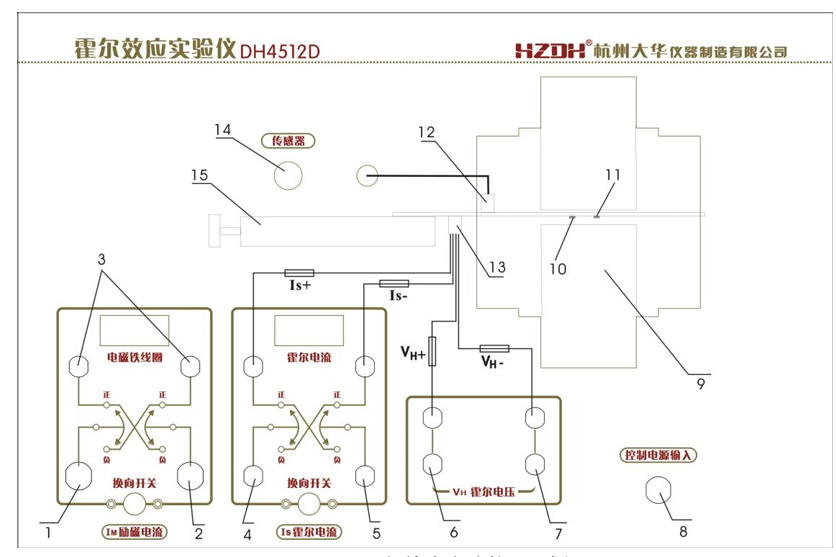
\includegraphics[width=0.8\textwidth]{test_stand_layout.png} % 在此处替换为你的图片文件名
    \caption{DH4512D 霍尔效应实验仪 测试架平面图}
    \label{fig:test_stand}
\end{figure}

\textbf{测试架组成部件说明：}
\begin{enumerate}
    \item 电磁铁励磁电流 $I_M$ 输入+（与测试仪对应 $I_M+$ 输出相连）
    \item 电磁铁励磁电流 $I_M$ 输入-（与测试仪对应 $I_M-$ 输出相连）
    \item 电磁铁线圈端（内部已连接到电磁铁线圈，无需再连线）
    \item 霍尔工作电流 $I_S+$ 输入（与测试仪对应 $I_S+$ 输出相连）
    \item 霍尔工作电流 $I_S-$ 输入（与测试仪对应 $I_S-$ 输出相连）
    \item 霍尔电压输出正极 $V_{H+}$（与测试仪对应 $V_H$ 输入相连）
    \item 霍尔电压输出负极 $V_{H-}$（与测试仪对应 $V_H$ 输入相连）
    \item 控制电源输入（继电器控制工作电源，与测试仪机箱后面板控制电源输出相连）
    \item 电磁铁（由铁芯和线圈组成，用于产生磁场）
    \item 霍尔元件（被测霍尔元件，用于研究其霍尔效应特性）
    \item 霍尔传感器（用于测量电磁铁磁场）
    \item 霍尔传感器信号输出插座，通过连接线内接到传感器插座 14 上
    \item 霍尔元件引脚插座（被测霍尔元件，共四线输出，分别为 $I_S+, I_S-, V_{H+}, V_{H-}$，每根线上均有号码管进行标示，连接时注意脚位）
    \item 霍尔传感器插座（与测试仪毫特计传感器插座相连）
    \item 可调移动尺，微调霍尔元件在电磁铁间隙中的位置
\end{enumerate}

\subsubsection{DH4512D 霍尔效应测试仪}

\begin{figure}[htbp]
    \centering
    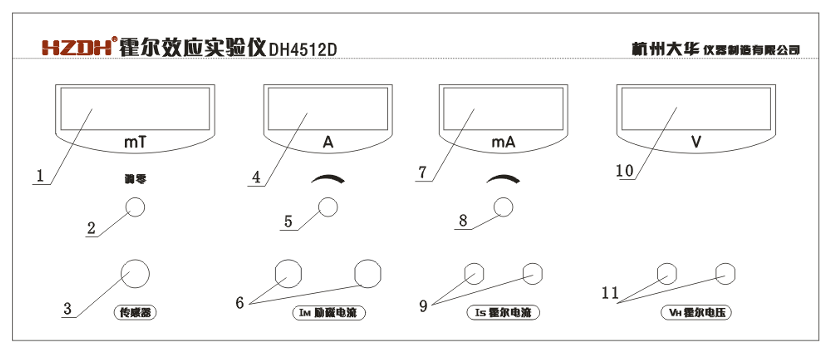
\includegraphics[width=0.8\textwidth]{panel_diagram.png} % 在此处替换为你的图片文件名
    \caption{DH4512D 霍尔效应实验仪 测试仪面板图}
    \label{fig:panel}
\end{figure}

\textbf{测试仪面板部件说明：}
\begin{itemize}
    \item \textbf{1.} 毫特计显示窗 \quad \textbf{2.} 毫特计调零电位器 \quad \textbf{3.} 毫特计传感器接口
    \item \textbf{4.} $I_M$ 励磁电流显示 \quad \textbf{5.} $I_M$ 励磁电流调节电位器 \quad \textbf{6.} $I_M$ 励磁电流输出接口
    \item \textbf{7.} $I_S$ 霍尔工作电流显示 \quad \textbf{8.} $I_S$ 霍尔工作电流调节电位器 \quad \textbf{9.} $I_S$ 霍尔工作电流输出
    \item \textbf{10.} 霍尔电压 $V_H$ 显示 \quad \textbf{11.} 霍尔电压 $V_H$ 输入接口
\end{itemize}

\subsubsection{使用说明}

\begin{enumerate}
    \item 测试仪的供电电源为交流 220V，50Hz，电源进线为单相三线。
    \item 电源插座安装在机箱背面，保险丝为 1A，置于电源插座内，电源开关在面板的左侧。
    \item 测试仪面板上的“$I_M$ 输出”、“$I_S$ 输出”和“$V_H$ 输入”三对接线柱应分别与测试架上的三对相应的接线柱正确连接。
    \item 将控制电源连接线一端插入测试仪背部的控制电源输出插孔，另一端连接到测试架的控制电源输入插孔。
    \item \textbf{仪器开机前}应将 $I_S$、$I_M$ 调节旋钮逆时针方向旋到底，使其输出电流趋于最小状态，然后再开机。
    \item 仪器接通电源后，预热数分钟即可进行实验。
    \item “$I_S$ 调节”和“$I_M$ 调节”分别来控制样品工作电流和励磁电流的大小，其电流随旋钮顺时针方向转动而增加，需细心操作。
    \item \textbf{关机前}，应将“$I_S$ 调节”和“$I_M$ 调节”旋钮逆时针方向旋到底，使其输出电流趋于零，然后才可切断电源。
    \item \textbf{继电器换向开关的使用说明}：
    \begin{itemize}
        \item 当未按下转换开关时，继电器线圈不加电，常闭端与动触点相连接；当按下按钮开关时，继电器吸合，常开端与动触点相连接，实现连接线的转换。由此可知，通过按下、按上转换开关，可以实现与继电器相连的连接线的换向功能。
        \item 本测试架内部定义：按下转换开关，上面两排指示灯亮，代表电流为正向；转换开关弹起时，下面两排指示灯亮，代表电流为负向。
    \end{itemize}
\end{enumerate}

\subsubsection{仪器主要技术性能}

\begin{enumerate}
    \item \textbf{电磁铁系统}：磁场可调范围 $0 \sim 350\,\text{mT}$，励磁电流 $0 \sim 0.5\,\text{A}$ 连续可调；调节细度 $< 1\,\text{mA}$，稳定性 $< 10^{-5}$；采用三位半数字电表显示。
    \item \textbf{数字式特斯拉计}：测量范围 $0 \sim 1000.0\,\text{mT}$，最小分辨率 $0.1\,\text{mT}$；采用四位半数字电表显示。
    \item \textbf{霍尔工作电流源}：输出电流 $0 \sim 3.5\,\text{mA}$ 连续可调，最小分辨率 $10\,\mu\text{A}$；采用三位半数字电表显示。
    \item \textbf{霍尔电压表}：量程 $0 \sim 2.0000\,\text{V}$，最小分辨率 $0.1\,\text{mV}$；采用四位半数字电表显示。
    \item \textbf{换向系统}：励磁电流和霍尔工作电流均采用电子换向开关。
    \item \textbf{位移机构}：可调移动尺调节范围为 $14\,\text{mm} \sim 44\,\text{mm}$。
\end{enumerate}

\subsection{亥姆霍兹线圈实验仪器与用具}

亥姆霍兹线圈磁感应强度实验仪由两个主要部分组成：亥姆霍兹线圈架部分（包括用于测量磁感应强度的感应线圈传感器盒）和磁感应强度测量仪（DH4501）。

\subsubsection{亥姆霍兹线圈架}

\begin{figure}[htbp]
    \centering
    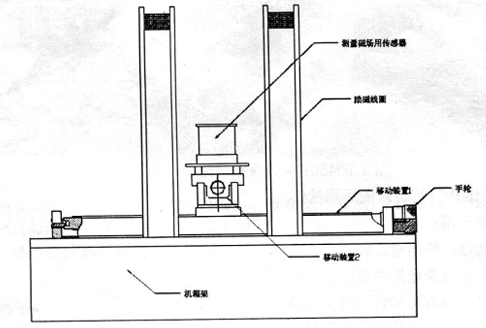
\includegraphics[width=0.8\textwidth]{figure4_coil_stand.png} % 请替换为实际文件名
     \caption{亥姆霍兹线圈架部分}
 \end{figure}

 \begin{figure}[htbp]
     \centering
     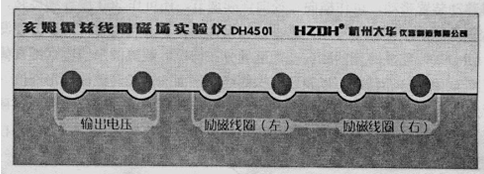
\includegraphics[width=0.8\textwidth]{figure5_panel.png} % 请替换为实际文件名
     \caption{DH4501 亥姆霍兹线圈架面板}
 \end{figure}

\subsubsection{DH4501 亥姆霍兹线圈磁感应强度测量仪}

 \begin{figure}[htbp]
     \centering
     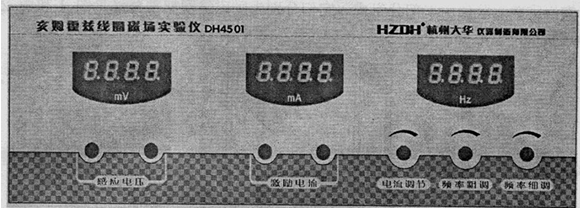
\includegraphics[width=0.8\textwidth]{figure6_instrument.png} % 请替换为实际文件名
     \caption{DH4501 亥姆霍兹线圈磁感应强度测量仪面板}
 \end{figure}

\subsubsection{主要技术指标}

\begin{enumerate}
    \item \textbf{亥姆霍兹线圈架}
    \begin{itemize}
        \item \textbf{二个励磁线圈}：线圈有效半径 $105\,\text{mm}$；单个线圈匝数 400 匝；二线圈中心间距 $105\,\text{mm}$。
        \item \textbf{移动装置}：轴向可移动距离 $250\,\text{mm}$；径向可移动距离 $70\,\text{mm}$；距离分辨率 $1\,\text{mm}$。
        \item \textbf{探测线圈}：匝数 1000 匝；旋转角度 360 度。
    \end{itemize}

    \item \textbf{DH4501 亥姆霍兹磁感应强度测量仪}
    \begin{itemize}
        \item \textbf{频率范围}：$20 \sim 200\,\text{Hz}$；频率分辨率：$0.1\,\text{Hz}$；测量误差：$0.1\%$。
        \item \textbf{正弦波}：输出电压幅度最大 $20\text{Vp-p}$；输出电流幅度最大 $200\,\text{mA}$。
        \item \textbf{数显毫伏表电压测量范围}：$0 \sim 20\,\text{mV}$；测量误差：$1\%$。
    \end{itemize}

    \item \textbf{电源}：$220\text{V} \pm 10\%$

    \item \textbf{外形尺寸}
    \begin{itemize}
        \item 亥姆霍兹线圈架：$340\,\text{mm} \times 270\,\text{mm} \times 250\,\text{mm}$
        \item 磁感应强度测量仪：$320\,\text{mm} \times 300\,\text{mm} \times 120\,\text{mm}$
    \end{itemize}
\end{enumerate}

\section{实验原理}
\subsection{霍尔效应实验原理及副效应的消除}

\subsubsection{霍尔效应原理}
霍尔效应是指运动的带电粒子在磁场中受洛伦兹力作用而发生偏转，从而在垂直于电流和磁场的方向上产生电势差的现象。

如图所示，当电流 $I_S$ 通过厚度为 $d$ 的半导体薄片，且磁感应强度 $B$ 垂直于薄片时，在薄片两侧产生的霍尔电势差 $V_H$ 为：
\begin{equation}
    V_H = K_H I_S B
\end{equation}
其中，$K_H$ 为霍尔元件的灵敏度，单位为 $[\text{mV}/\text{mA}\cdot\text{T}]$。它与材料的性质及几何尺寸有关：
\begin{equation}
    K_H = \frac{R_H}{d} = \frac{1}{n e d}
\end{equation}
式中 $n$ 为载流子浓度，$e$ 为电子电量。

\subsubsection{副效应及其消除方法}
在实际测量中，霍尔电极两端输出的电压 $V_{AB}$ 不仅包含霍尔电压 $V_H$，还叠加了多种副效应产生的附加电压，主要包括：
\begin{itemize}
    \item \textbf{不等位电势 $V_0$}：由电极不对称或材料电阻不均匀引起（与 $I_S$ 有关，与 $B$ 无关）；
    \item \textbf{爱廷豪森效应 $V_E$}：载流子偏转引起的温差电动势（与 $I_S B$ 成正比，极性与 $V_H$ 相同）；
    \item \textbf{伦斯脱效应 $V_N$}：纵向温度梯度引起的温差电动势（只与 $B$ 有关）；
    \item \textbf{里纪-杜勒克效应 $V_R$}：热扩散引起的温差电动势（只与 $B$ 有关）。
\end{itemize}

为消除上述副效应（除 $V_E$ 外），实验采用\textbf{对称测量法}（交换法）。即依次改变工作电流 $I_S$ 和磁场 $B$ 的方向，在四种组合下测量电压：
\begin{align}
    V_1 (+I_S, +B) &= +V_H + V_0 + V_E + V_N + V_R \\
    V_2 (+I_S, -B) &= -V_H + V_0 - V_E + V_N + V_R \\
    V_3 (-I_S, -B) &= +V_H - V_0 + V_E - V_N - V_R \\
    V_4 (-I_S, +B) &= -V_H - V_0 - V_E - V_N - V_R
\end{align}
通过代数运算可消除大部分系统误差：
\begin{equation}
    V_H + V_E = \frac{1}{4}(V_1 - V_2 + V_3 - V_4)
\end{equation}
由于在非大电流和弱磁场下，爱廷豪森效应 $V_E \ll V_H$，通常可忽略不计，故霍尔电压可近似为：
\begin{equation}
    V_H \approx \frac{V_1 - V_2 + V_3 - V_4}{4}
\end{equation}

\subsection{亥姆霍兹线圈实验原理}

\subsubsection{载流圆线圈的磁感应强度}

一半径为 $R$，通以电流 $I$ 的圆线圈，轴线上磁感应强度的公式为：
\begin{equation}
    B = \frac{\mu_0 N_0 I R^2}{2(R^2 + X^2)^{3/2}} \label{eq:single_coil_B}
\end{equation}
式中 $N_0$ 为圆线圈的匝数，$\text{X}$ 为轴上某一点到圆心 0 的距离。$\mu_0 = 4\pi \times 10^{-7} \, \text{H/m}$。轴线上磁感应强度的分布如图 \ref{fig:single_coil} 所示。

\begin{figure}[htbp]
    \centering
    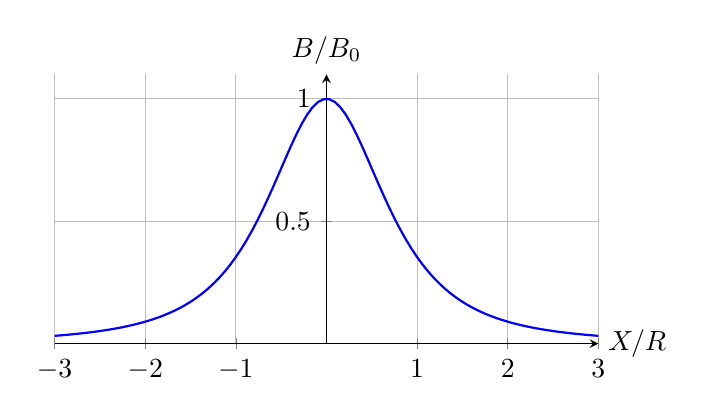
\begin{tikzpicture}
        \begin{axis}[
            width=0.7\textwidth,
            height=5cm,
            xlabel={$X/R$},
            ylabel={$B/B_0$},
            xmin=-3, xmax=3,
            ymin=0, ymax=1.1,
            grid=major,
            domain=-3:3,
            samples=100,
            axis lines=middle,
            every axis x label/.style={at={(current axis.right of origin)},anchor=west},
            every axis y label/.style={at={(current axis.above origin)},anchor=south},
        ]
        \addplot[blue, thick] {1/(1+x^2)^1.5};
        \end{axis}
    \end{tikzpicture}
    \caption{单个圆环线圈的磁感应强度分布示意图}
    \label{fig:single_coil}
\end{figure}

本实验取 $N_0=400$ 匝，$R=105\text{mm}$。当 $f=120\text{Hz}$，$I=60\text{mA}$（有效值），圆心 0 处 $\text{X}=0$，可计算得到单个圆线圈中的磁感应强度为：$B=0.144\text{mT}$。

\subsubsection{亥姆霍兹线圈的磁感应强度}

所谓亥姆霍兹线圈为两个相同线圈彼此平行且共轴，使线圈上通以相同方向电流 I，理论计算证明：线圈距离 $a$ 等于线圈半径 $R$ 时，两个单个线圈的磁感应强度叠加在轴上（两个线圈的圆心连线）附近较大范围内的合磁感应强度是均匀的，如图 \ref{fig:helmholtz_coil} 所示。

\begin{figure}[htbp]
    \centering
    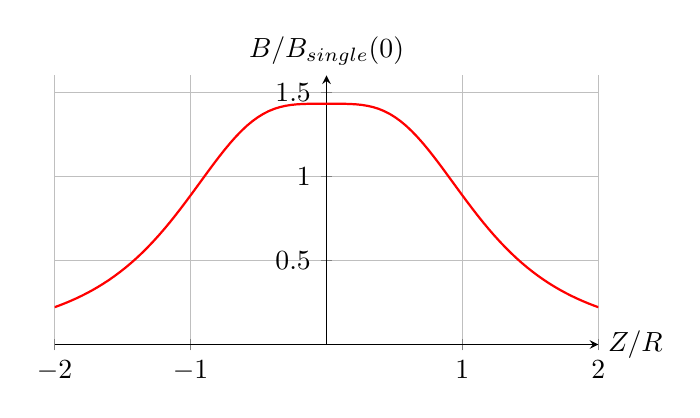
\begin{tikzpicture}
        \begin{axis}[
            width=0.7\textwidth,
            height=5cm,
            xlabel={$Z/R$},
            ylabel={$B/B_{single}(0)$},
            xmin=-2, xmax=2,
            ymin=0, ymax=1.6,
            grid=major,
            domain=-2:2,
            samples=100,
            axis lines=middle,
            every axis x label/.style={at={(current axis.right of origin)},anchor=west},
            every axis y label/.style={at={(current axis.above origin)},anchor=south},
        ]
        \addplot[red, thick] { (1+(0.5+x)^2)^(-1.5) + (1+(0.5-x)^2)^(-1.5) };
        \end{axis}
    \end{tikzpicture}
    \caption{亥姆霍兹线圈的磁感应强度分布示意图}
    \label{fig:helmholtz_coil}
\end{figure}

设 $Z$ 为亥姆霍兹线圈中轴线上某一点离中心点 O 处的距离，则亥姆霍兹线圈轴线上改点的磁感应强度为：
\begin{equation}
    B = \frac{1}{2} \mu_0 N I R^2 \left\{ \left[ R^2 + \left(\frac{R}{2} + z\right)^2 \right]^{-\frac{3}{2}} + \left[ R^2 + \left(\frac{R}{2} - z\right)^2 \right]^{-\frac{3}{2}} \right\} \label{eq:helmholtz_B_z}
\end{equation}
而在亥姆霍兹线圈轴线上中心 O 处，$Z=0$，磁感应强度为
\begin{equation}
    B = \frac{\mu_0 N_0 I}{2R} \times \frac{16}{5^{3/2}} \label{eq:helmholtz_B_0}
\end{equation}
当实验取 $N_0=400$ 匝，$R=105\text{mm}$。当 $f=120\text{Hz}$，$I=60\text{mA}$（有效值）时，在中心 0 处 $Z=0$，可计算得到亥姆霍兹线圈（两个线圈的合成）磁感应强度为：
\[
B = \frac{\mu_0 N_0 I}{2R} \times \frac{16}{5^{3/2}} = 1.43 \times 1.431 = 2.05\text{mT}
\]

\subsubsection{电磁感应测量原理}

设由交流信号驱动的线圈产生的交变磁感应强度，它的磁感应强度的瞬时值为
\[
B = B_m \sin \omega t
\]
式中 $B_m$ 为磁感应强度的峰值，其有效值记作 $B$，$\omega$ 为角频率。磁感应强度中一探测线圈的磁通量为
\[
\Phi = N S B_m \cos \theta \sin \omega t
\]
式中：$N$ 为探测线圈的匝数，$S$ 为该线圈的截面积，$\theta$ 为 $B$ 与线圈法线夹角。线圈产生的感应电动势为
\[
\varepsilon = - \frac{d\Phi}{dt} = N S \omega B_m \cos \theta \cos \omega t
\]
\[
= - \varepsilon_m \cos \omega t
\]
式中 $\varepsilon_m = N S \omega B_m \cos \theta$ 是线圈法线和磁感应强度成 $\theta$ 角时，感应电动势的幅值。当 $\theta = 0$，$\varepsilon_{max} = N S \omega B_m$，这时的感应电动势的幅值最大。如果用数字式毫伏表测量此时线圈的电动势，则毫伏表的示值（有效值）$U_{\max}$ 为 $\frac{\varepsilon_{max}}{\sqrt{2}}$，则
\begin{equation}
    B_{\max} = \frac{\varepsilon_{\max}}{NS\omega} = \frac{\sqrt{2} U_{\max}}{NS\omega} \label{eq:Bm_calc}
\end{equation}
$B$ 为磁感应强度有效值，$B_m$ 为磁感应强度的峰值。由式 \eqref{eq:Bm_calc} 可计算出 $B_m$ 来。

\subsubsection{探测线圈的设计}

实验中由于磁感应强度的不均匀性，探测线圈又不可能做得很大，否则会影响测量灵敏度。一般设计的线圈长度 $L$ 和外径 $D$ 有 $L=2/3 D$ 的关系，线圈的内径 $d$ 与外径 $D$ 有 $d \le 3/D$ 的关系（本实验选 $D=0.012\text{m}$，$N=800$ 匝的线圈）。线圈在磁感应强度中的等效面积，经过理论计算，可用下式表示
\begin{equation}
    S = \frac{13}{108} \pi D^2 \label{eq:coil_area}
\end{equation}
这样的线圈测得的平均磁感应强度可以近似看成是线圈中心点的磁感应强度。本实验励磁电流由专用的交变磁感应强度测试仪提供。
\begin{equation}
    B = \frac{54}{13 \pi^2 N D^2 f} U_{max} \label{eq:B_final}
\end{equation}
将不同的频率 $f$ 代入上式就可以得出 $B$。本实验的 $D=0.012\text{m}$，$N=1000$ 匝。
例如，$I=60\text{mA}$，$f=120\text{Hz}$ 时，交流毫伏表读数为 $5.95\text{mV}$，则根据式 \eqref{eq:B_final} 求得单个线圈的磁感应强度 $B=0.145\text{mT}$。

\section{实验内容}

\subsection{注意事项}

\begin{enumerate}
    \item 当霍尔片未连接到实验架，并且实验架与测试仪未连接好时，严禁开机加电，防止霍尔片遭受冲击电流而损坏。
    \item 霍尔片性脆易碎、电极易断，严禁用手去触摸，以免损坏。
    \item 加电前必须保证测试仪的“$I_S$ 调节”和“$I_M$ 调节”旋钮均置零位（即逆时针旋转到底），未调零不可开机。
    \item 测试仪的“$I_S$ 输出”接实验架的“$I_S$ 输入”，“$I_M$ 输出”接“$I_M$ 输入”。不可混接，否则一旦通电，会因电流过大损坏霍尔片。
    \item 为了不使电磁铁线圈过热而受到损害，或影响测量精度，除在短时间内读取有关数据外，其余时间最好断开 $I_M$ 励磁电流或者调到最小。
    \item 移动尺的调节范围有限。在调节到两边停止移动后，不可继续调节，以免因错位而损坏移动尺。
    \item 接线或测量数据时，要特别注意检查移动两个线圈时，是否满足亥姆霍兹线圈的条件。
    \item 两个线圈采用串接或并接方式与电源相连时，必须注意磁感应强度的方向。如果接错线有可能使亥姆霍兹线圈中间轴线上磁感应强度为零。
    \item 改变线圈电流频率时，注意调整电流不变。
\end{enumerate}

\subsection{利用霍尔效应实验仪测量磁感应强度}

\begin{enumerate}
    \item 测量 $V_H$ 与 $I_S$ 的关系：
    \begin{itemize}
        \item 将霍尔效应测试仪与测试架正确连接。检查测试仪的“$I_S$ 调节”和“$I_M$ 调节”旋钮是否均置零位。用移动尺将霍尔元件移至电磁铁中心，在 $I_M=0$ 的情况下，用调零旋钮调零毫特斯拉计。
        \item 调节 $I_M=200\text{mA}$，按转换开关切换电流方向，测量霍尔电压 $V_1, V_2, V_3, V_4$ 的值。按下转换开关，上面两排指示灯亮，代表电流为正向；转换开关弹起时，下面两排指示灯亮，代表电流为负向。
        \item $I_S$ 每次递增 $0.5\text{mA}$，测量霍尔电压 $V_1, V_2, V_3, V_4$ 的值。
    \end{itemize}

    \item 测量 $V_H$ 与 $B$ 的关系、$B$ 与 $I_M$ 的关系
    \begin{itemize}
        \item 将 $I_M, I_S$ 调零，用调零旋钮调零毫特斯拉计，再调节 $I_S=1\text{mA}$，测量 4 种电流方向下霍尔电压 $V_H$ 与磁感应强度 $B$ 的值。
        \item $I_M$ 每次递增 $50\text{mA}$，测量 4 种电流方向下霍尔电压 $V_H$ 与磁感应强度 $B$ 的值。
        \item 计算霍尔元件的灵敏度：\\
        作出 $V_H - B$ 图像，由最小二乘法得出线性拟合曲线的斜率 $K_{H-B}$，由 (5) 得到：
        \begin{equation}
            K_H = \frac{K_{H-B}}{I_S} \tag{20}
        \end{equation}
        并与理论值相比较。
    \end{itemize}

    \item 测量水平方向电磁铁磁场分布
    \begin{itemize}
        \item 在 $I_M=0$ 的情况下，用调零旋钮调零毫特斯拉计。
        \item 调节 $I_M=200\text{mA}$，记录毫特斯拉计示数 $B$。
        \item 调节移动尺位置，每 $2\text{mm}$ 记录一次毫特斯拉计示数 $B$。
    \end{itemize}

    \item 交流霍尔电流测量磁场
    \begin{itemize}
        \item 用函数发生器代替直流稳压电源产生交流霍尔电流 $I_{S-AC}$，台式万用表测量霍尔电压，数字万用表调节为毫安挡交流模式测定交流霍尔电流，连接好实验电路，如图：
        \begin{figure}[htbp]
            \centering
            \begin{minipage}[b]{0.48\textwidth}
                \centering
                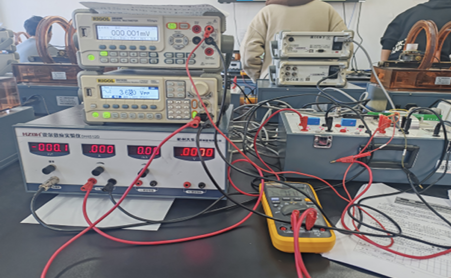
\includegraphics[width=\textwidth]{image_a.png} % 请替换为实际图片路径
                \caption{ 交流霍尔电流测磁场实物电路正视图}
            \end{minipage}
            \hfill
            \begin{minipage}[b]{0.48\textwidth}
                \centering
                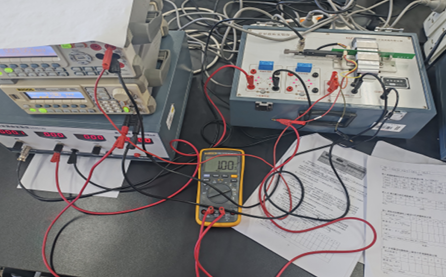
\includegraphics[width=\textwidth]{image_b.png} % 请替换为实际图片路径
                \caption{交流霍尔电流测磁场实物电路俯视图}
            \end{minipage}
        \end{figure}

        \item 设置函数发生器输出正弦波频率 $f=500\text{Hz}$，调节输出电压幅值使得数字万用表显示交流霍尔电流有效值 $I_{S-AC}=1\text{mA}$。霍尔电流设置好后，台式万用表接入霍尔电压。
        \item 调节励磁电流 $I_M$ 从 $50\text{mA}$ 开始，每 $25\text{mA}$，记录相应的毫特斯拉计示数 $B$ 和交流台式电压表示数 $V_{H-AC}$，作出 $B-I_M$ 图，并计算灵敏度 $K_H$，与理论值相比较。
    \end{itemize}
\end{enumerate}

\subsection{亥姆霍兹线圈的磁感应强度测量}

\begin{enumerate}
    \item 测量圆电流线圈轴线上磁感应强度的分布
    \begin{itemize}
        \item 开机预热 10 分钟，并连接好器材线路。
        \item 在励磁电流为零的情况下调零毫伏电压表。调节频率调节电位器为 $120\text{Hz}$。调节电流调节电位器，使励磁电流有效值为 $I=60\text{mA}$。调节探测线圈法线方向与圆电流线圈轴线夹角为 $0^\circ$。此时毫伏电压表的示数即为该处的 $U_{max}$。\\
        ($0^\circ$ 和 $180^\circ$ 都是最大值，但在实验中往往不相等，可以预先测出两个数据，若正反方向测量误差不大，2\%，则任取一个方向数据。否则取平均值。)
        \item 转动探测线圈轴向调节手轮，以圆电流线圈中心为坐标原点，每隔 $5\text{mm}$ 测一个 $U_{max}$ 值，测量过程中注意保持励磁电流值不变。
    \end{itemize}

    \item 测量亥姆霍兹线圈轴线上磁感应强度的分布
    \begin{itemize}
        \item 连接好实验电路。在励磁电流为零的情况下调零毫伏电压表。
        \item 保持励磁电流频率为 $120\text{Hz}$、有效值为 $I=60\text{mA}$ 不变。
        \item 转动探测线圈轴向调节手轮，以亥姆霍兹线圈中心为坐标原点，每隔 $5\text{mm}$ 测一个 $U_{max}$ 值。
    \end{itemize}

    \item 测量亥姆霍兹线圈沿径向的磁感应强度分布
    \begin{itemize}
        \item 保持探测线圈法线方向与轴线夹角为 $0^\circ$，励磁电流频率为 $120\text{Hz}$、有效值为 $I=60\text{mA}$ 不变。
        \item 转动探测线圈径向调节手轮，以亥姆霍兹线圈中心为坐标原点，每隔 $5\text{mm}$ 测一个 $U_{max}$ 值，按正负方向测到边缘。
    \end{itemize}

    \item 验证 $\varepsilon_m(\theta) = N S B_m \omega \cos\theta$
    \begin{itemize}
        \item 把探测线圈沿轴线固定在某一位置上
        \item 转动传感器盒的有机玻璃罩，使探测线圈法线方向（玻璃罩上有画线）与轴线的夹角从 $0^\circ$ 开始旋转一周，每改变 $10^\circ$ 测一组电压值。
    \end{itemize}

    \item 励磁电流频率大小对磁感应强度的影响
    \begin{itemize}
        \item 把探测线圈固定在亥姆霍兹线圈中心点，保持法线方向与轴线的夹角为 $0^\circ$ 不变。
        \item 调节输出电流频率，$20\text{Hz} \sim 150\text{Hz}$ 范围内每次改变 $10\text{Hz}$，逐次测量感应电动势的数值并记录。
    \end{itemize}
\end{enumerate}

\section{数据处理与分析}
\subsection{利用霍尔效应实验仪测量磁感应强度}
\subsubsection{测量$V_H$与$I_S$的关系}
实验数据记录如下\ref{tab:hall_effect_data}：
 \begin{table}[htbp]
    \centering
    \caption{霍尔电压 $V_H$ 与工作电流 $I_S$ 数据记录 ($I_M = 200\text{mA}$)}
    \label{tab:hall_effect_data}
    \begin{tabular}{cccccc}
        \toprule
        \multirow{2}{*}{$I_S (\text{mA})$} & $V_1 (\text{mV})$ & $V_2 (\text{mV})$ & $V_3 (\text{mV})$ & $V_4 (\text{mV})$ & \multirow{2}{*}{$V_H = \frac{V_1 - V_2 + V_3 - V_4}{4} (\text{mV})$} \\
        % 第二行表头：表示电流方向
         & $+I_M +I_S$ & $+I_M -I_S$ & $-I_M -I_S$ & $-I_M +I_S$ & \\
        \midrule
        0       & 0        & 0         & 0        & 0         & 0       \\
        0.50    & 0.0226   & $-0.0224$ & 0.0298   & $-0.0297$ & 0.0261  \\
        1.00    & 0.0446   & $-0.0441$ & 0.0587   & $-0.0586$ & 0.0515  \\
        1.50    & 0.0667   & $-0.0659$ & 0.0876   & $-0.0876$ & 0.0770  \\
        2.00    & 0.0891   & $-0.0882$ & 0.1170   & $-0.1170$ & 0.1028  \\
        2.50    & 0.1111   & $-0.1100$ & 0.1456   & $-0.1462$ & 0.1282  \\
        3.00    & 0.1337   & $-0.1324$ & 0.1749   & $-0.1756$ & 0.1542  \\
        \bottomrule
    \end{tabular}
\end{table}

\begin{figure}[htbp]
    \centering
    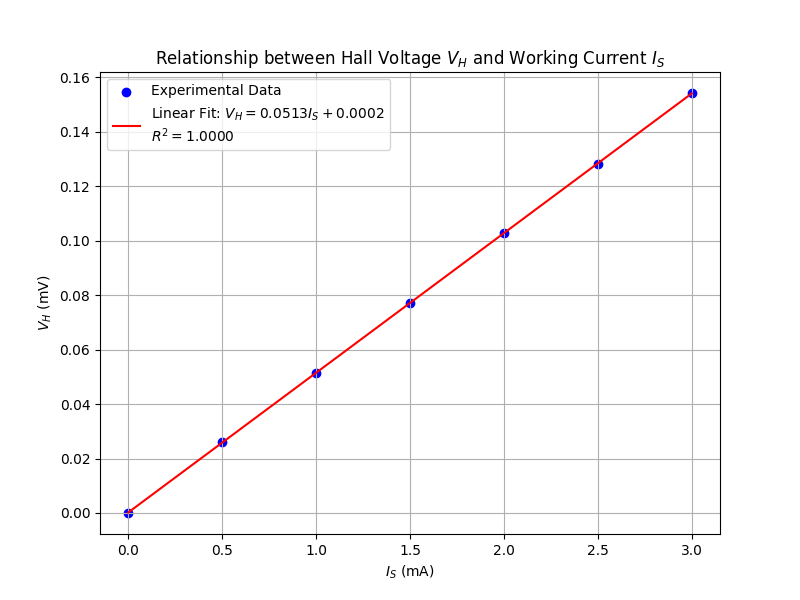
\includegraphics[width=0.7\textwidth]{VH_vs_IS_plot.png}
    \caption{$V_H - I_S$ 关系曲线及线性拟合}
    \label{fig:VH_IS_plot}
\end{figure}

\textbf{结果分析：}

根据实验数据绘制 $V_H - I_S$ 关系图如图 \ref{fig:VH_IS_plot} 所示。利用最小二乘法对数据进行线性拟合，得到拟合方程为：
\begin{equation}
    V_H = 0.0513 I_S + 0.0002
\end{equation}
相关系数 $R^2 = 0.99999$，表明 $V_H$ 与 $I_S$ 具有极好的线性关系。截距 $0.0002\,\text{mV}$ 接近于零，符合霍尔效应原理公式 $V_H = K_H I_S B$（当 $B$ 一定时，$V_H \propto I_S$）。实验结果验证了在磁场恒定的情况下，霍尔电压与工作电流成正比。

\subsubsection{测量$V_H$与$I_M$的关系,测量$B$与$I_M$的关系}

\begin{table}[htbp]
    \centering
    \caption{霍尔电压 $V_H$ 与励磁电流 $I_M$ 数据记录 ($V_H - I_M$, $I_S = 1.00\text{mA}$)}
    \label{tab:hall_effect_im}
    \begin{tabular}{cccccc}
        \toprule
        \multirow{2}{*}{$I_M (\text{mA})$} & $V_1 (\text{mV})$ & $V_2 (\text{mV})$ & $V_3 (\text{mV})$ & $V_4 (\text{mV})$ & \multirow{2}{*}{$V_H = \frac{V_1 - V_2 + V_3 - V_4}{4} (\text{mV})$} \\
         & $+I_M +I_S$ & $+I_M -I_S$ & $-I_M -I_S$ & $-I_M +I_S$ & \\
        \midrule
        0   & $-0.0070$ & $0.0069$  & $0.0070$ & $-0.0070$ & 0.0000 \\
        50  & $0.0056$  & $-0.0056$ & $0.0200$ & $-0.0201$ & 0.0128 \\
        100 & $0.0186$  & $-0.0186$ & $0.0330$ & $-0.0330$ & 0.0258 \\
        150 & $0.0316$  & $-0.0316$ & $0.0459$ & $-0.0461$ & 0.0388 \\
        200 & $0.0447$  & $-0.0444$ & $0.0590$ & $-0.0590$ & 0.0518 \\
        250 & $0.0576$  & $-0.0579$ & $0.0722$ & $-0.0724$ & 0.0650 \\
        300 & $0.0709$  & $-0.0709$ & $0.0852$ & $-0.0853$ & 0.0781 \\
        \bottomrule
    \end{tabular}
\end{table}
\begin{figure}[htbp]
    \centering
    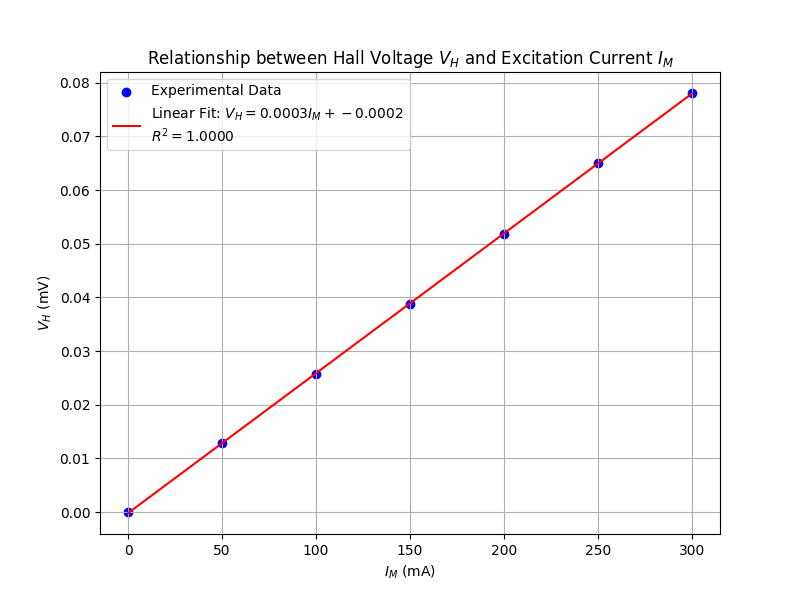
\includegraphics[width=0.7\textwidth]{VH_vs_IM_plot.png}
    \caption{$V_H - I_M$ 关系曲线及线性拟合}
    \label{fig:VH_IM_plot}
\end{figure}

\textbf{结果分析：}

根据实验数据绘制 $V_H - I_M$ 关系图如图 \ref{fig:VH_IM_plot} 所示。利用最小二乘法对数据进行线性拟合，得到拟合方程为：
\begin{equation}
    V_H = 0.00026 I_M - 0.0002
\end{equation}
相关系数 $R^2 = 0.99998$，B表明 $V_H$ 与 $I_M$ 具有极好的线性关系。由于电磁铁产生的磁感应强度 $B$ 与励磁电流 $I_M$ 成正比（在未饱和区域），而 $V_H \propto B$，因此 $V_H$ 与 $I_M$ 应成正比。实验结果验证了这一点。



\begin{table}[htbp]
    \centering
    \caption{磁感应强度 $B$ 与励磁电流 $I_M$ 数据记录 ($B-I_M$, $I_S = 1.00\text{mA}$)}
    \label{tab:magnetic_induction}
    \begin{tabular}{cccccc}
        \toprule
        \multirow{2}{*}{$I_M (\text{mA})$} & $B_1 (\text{mT})$ & $B_2 (\text{mT})$ & $B_3 (\text{mT})$ & $B_4 (\text{mT})$ & \multirow{2}{*}{$B = \frac{B_1 + B_2 - B_3 - B_4}{4} (\text{mT})$} \\
         & $+I_M +I_S$ & $+I_M -I_S$ & $-I_M -I_S$ & $-I_M +I_S$ & \\
        \midrule
        0   & 0     & 0     & 0      & 0      & 0      \\
        50  & 36.7  & 36.7  & $-37.5$  & $-37.0$  & 36.98  \\
        100 & 73.9  & 73.7  & $-74.7$  & $-74.7$  & 74.25  \\
        150 & 110.7 & 111.9 & $-112.1$ & $-112.1$ & 111.70 \\
        200 & 148.4 & 147.6 & $-149.5$ & $-148.8$ & 148.58 \\
        250 & 185.4 & 186.3 & $-187.1$ & $-187.3$ & 186.53 \\
        300 & 223.5 & 223.6 & $-224.5$ & $-224.5$ & 224.03 \\
        \bottomrule
    \end{tabular}
\end{table}

\begin{figure}[htbp]
    \centering
    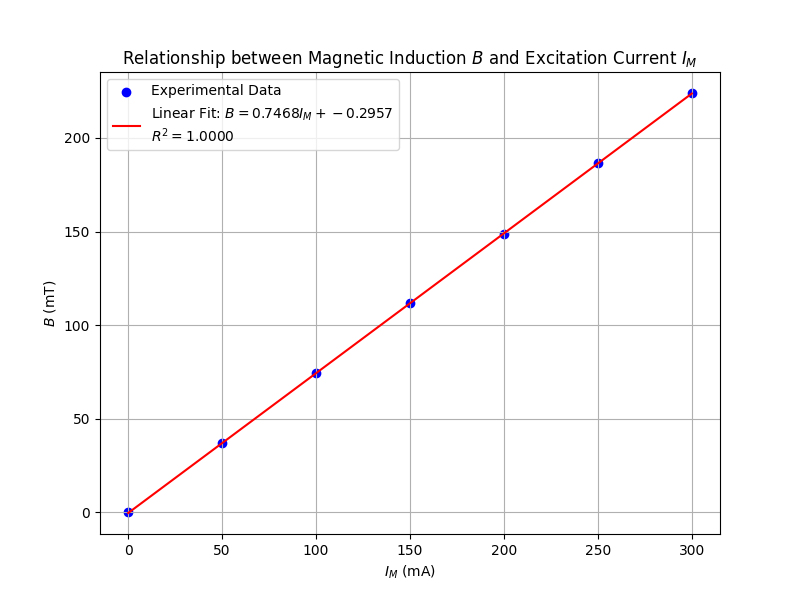
\includegraphics[width=0.7\textwidth]{B_vs_IM_plot.png}
    \caption{$B - I_M$ 关系曲线及线性拟合}
    \label{fig:B_IM_plot}
\end{figure}

\textbf{结果分析：}

根据实验数据绘制 $B - I_M$ 关系图如图 \ref{fig:B_IM_plot} 所示。利用最小二乘法对数据进行线性拟合，得到拟合方程为：
\begin{equation}
    B = 0.7468 I_M - 0.2957
\end{equation}
相关系数 $R^2 = 0.99999$，表明磁感应强度 $B$ 与励磁电流 $I_M$ 具有极好的线性关系。这说明在实验选取的电流范围内（$0 \sim 300\,\text{mA}$），电磁铁工作在磁化曲线的线性区域，未出现磁饱和现象。

\paragraph{霍尔灵敏度 $K_H$ 的计算与误差分析}

根据霍尔效应原理公式 $V_H = K_H I_S B$，可以通过实验数据的线性拟合斜率来计算霍尔灵敏度 $K_H$。

1. \textbf{由 $V_H - I_S$ 关系计算 $K_H$}：\\
在 $I_M = 200\,\text{mA}$ 时，由 $B - I_M$ 测量数据可知磁感应强度 $B = 148.58\,\text{mT} = 0.14858\,\text{T}$。
$V_H - I_S$ 拟合直线的斜率为 $k_1 = 0.0513\,\text{V/mA}$。
则：
\begin{equation}
    K_{H1} = \frac{k_1}{B} = \frac{0.0513}{0.14858} \approx 345.27\,\text{mV}/(\text{mA}\cdot\text{T})
\end{equation}

2. \textbf{由 $V_H - I_M$ 和 $B - I_M$ 关系计算 $K_H$}：\\
$V_H - I_M$ 拟合直线的斜率为 $k_2 = 0.00026\,\text{V/mA}$。
$B - I_M$ 拟合直线的斜率为 $k_B = 0.7468\,\text{mT/mA} = 0.0007468\,\text{T/mA}$。
在 $I_S = 1.00\,\text{mA}$ 时，有 $k_2 = K_H I_S k_B$，则：
\begin{equation}
    K_{H2} = \frac{k_2}{I_S \cdot k_B} = \frac{0.00026}{1.00 \times 0.0007468} \approx 348.15\,\text{mV}/(\text{mA}\cdot\text{T})
\end{equation}

3. \textbf{结果与误差分析}：\\
取两次计算的平均值作为实验测量值：
\begin{equation}
    \bar{K}_H = \frac{345.27 + 348.15}{2} = 346.71\,\text{mV}/(\text{mA}\cdot\text{T})
\end{equation}
已知霍尔灵敏度的理论值为 $K_{H\text{理论}} = 345\,\text{mV}/(\text{mA}\cdot\text{T})$，则相对误差为：
\begin{equation}
    E = \frac{|\bar{K}_H - K_{H\text{理论}}|}{K_{H\text{理论}}} \times 100\% = \frac{|346.71 - 345|}{345} \times 100\% \approx 0.50\%
\end{equation}

\textbf{误差来源分析：}
\begin{enumerate}
    \item \textbf{仪器误差}：数字万用表、毫特斯拉计等测量仪器存在固有的精度限制和读数误差。
    \item \textbf{温度影响}：霍尔元件的灵敏度 $K_H$ 会随温度变化，实验过程中电流通过元件会产生热量，导致温度升高，从而引入误差。
    \item \textbf{位置误差}：霍尔元件可能未完全置于电磁铁气隙的中心均匀磁场区域，或者霍尔片平面与磁场方向未完全垂直。
    \item \textbf{副效应消除不彻底}：虽然采用了对称交换测量法，但由于电流和磁场调节的微小偏差，可能无法完全消除所有副效应的影响。
\end{enumerate}

\subsubsection{测量水平方向电磁铁磁场分布}
\begin{table}[htbp]
    \centering
    \caption{电磁铁磁场沿水平方向分布数据记录 ($I_M = 200\text{mA}$)}
    \label{tab:magnetic_distribution_horizontal}
    \begin{tabular}{cccccccc}
        \toprule
        $X (\text{mm})$ & 42 & 40 & 38 & 36 & 34 & 32 & 30 \\
        $B (\text{mT})$ & 35.2 & 62.2 & 121.8 & 148.1 & 148.8 & 148.7 & 148.9 \\
        \midrule
        $X (\text{mm})$ & 28 & 26 & 24 & 22 & 20 & 18 & 16 \\
        $B (\text{mT})$ & 148.8 & 148.6 & 148.8 & 148.6 & 148.6 & 148.9 & 149.0 \\
        \bottomrule
    \end{tabular}
\end{table}

\begin{figure}[htbp]
    \centering
    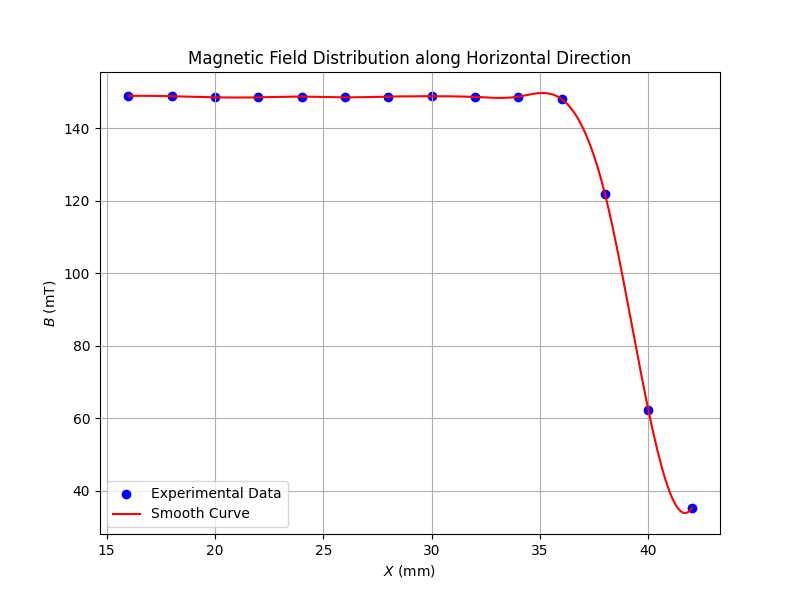
\includegraphics[width=0.8\textwidth]{plot_B_X.png}
    \caption{电磁铁磁场沿水平方向分布曲线}
    \label{fig:B_X}
\end{figure}

根据表 \ref{tab:magnetic_distribution_horizontal} 中的数据，绘制电磁铁磁场沿水平方向的分布曲线如图 \ref{fig:B_X} 所示。
从图中可以看出，在 $X \in [16, 34]\,\text{mm}$ 的范围内，磁感应强度 $B$ 基本保持恒定，约为 $148.8\,\text{mT}$，表明该区域为均匀磁场区。当 $X > 34\,\text{mm}$ 时，磁感应强度迅速下降，表明已移出均匀磁场区域。

\subsubsection{测量交流霍尔电流测量磁场}
\begin{table}[htbp]
    \centering
    \caption{AC 模式霍尔效应测量磁场 ($I_{S-AC}=1\text{mA}$)}
    \label{tab:ac_mode_hall}
    \begin{tabular}{cccccccc}
        \toprule
        $I_M (\text{mA})$ & 50 & 75 & 100 & 125 & 150 & 175 & 200 \\
        \midrule
        $B (\text{mT})$ & 37.3 & 55.5 & 74.1 & 92.9 & 111.2 & 130.6 & 148.4 \\
        $V_{H-AC} (\text{mV})$ & 6.371 & 12.488 & 18.909 & 25.435 & 31.755 & 38.547 & 44.637 \\
        \bottomrule
    \end{tabular}
\end{table}

\begin{figure}[htbp]
    \centering
    \begin{minipage}[t]{0.48\textwidth}
        \centering
        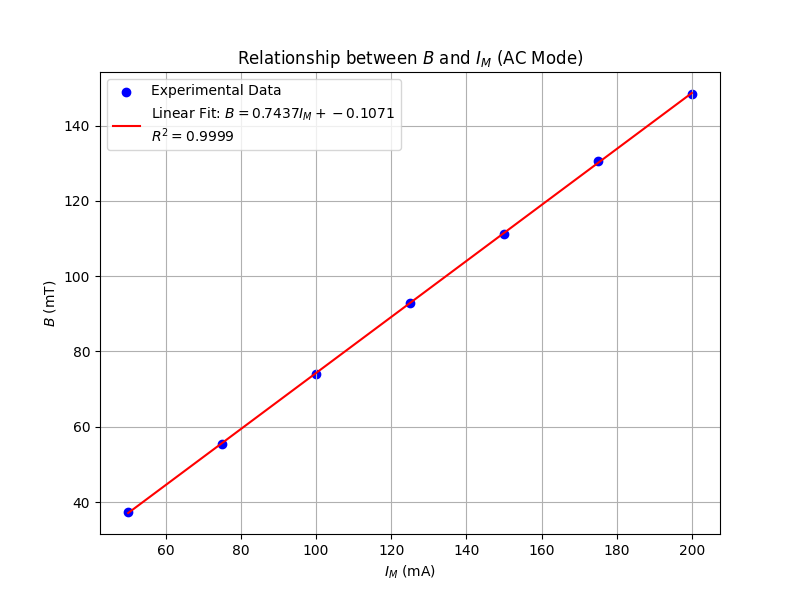
\includegraphics[width=\textwidth]{plot_AC_B_IM.png}
        \caption{AC模式下磁感应强度 $B$ 与励磁电流 $I_M$ 的关系}
        \label{fig:AC_B_IM}
    \end{minipage}
    \hfill
    \begin{minipage}[t]{0.48\textwidth}
        \centering
        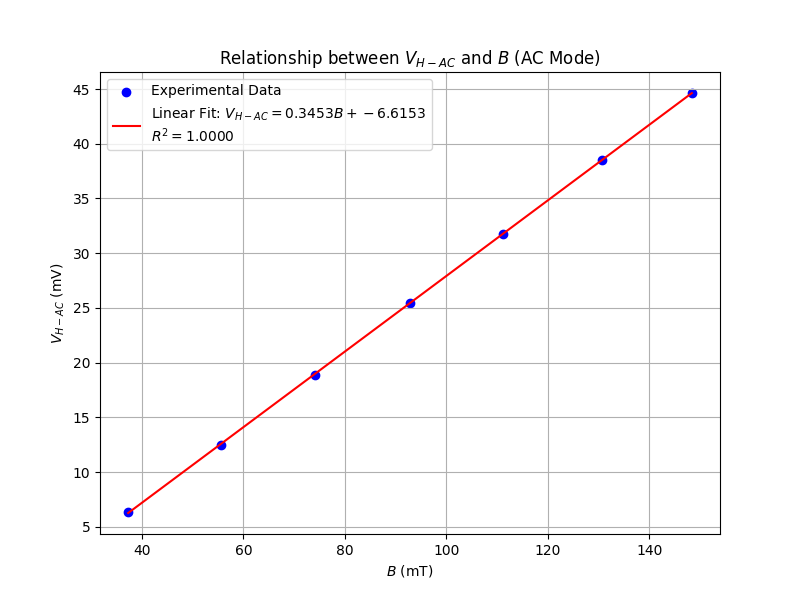
\includegraphics[width=\textwidth]{plot_AC_VH_B.png}
        \caption{AC模式下霍尔电压 $V_{H-AC}$ 与磁感应强度 $B$ 的关系}
        \label{fig:AC_VH_B}
    \end{minipage}
\end{figure}

根据表 \ref{tab:ac_mode_hall} 中的数据，分别绘制 $B$ 与 $I_M$ 以及 $V_{H-AC}$ 与 $B$ 的关系曲线，并进行线性拟合，如图 \ref{fig:AC_B_IM} 和 \ref{fig:AC_VH_B} 所示。

由图 \ref{fig:AC_B_IM} 可知，$B$ 与 $I_M$ 呈现良好的线性关系，拟合方程为：
\begin{equation}
    B = 0.7437 I_M - 0.1071 \quad (R^2 = 0.9999)
\end{equation}

由图 \ref{fig:AC_VH_B} 可知，$V_{H-AC}$ 与 $B$ 也呈现良好的线性关系，拟合方程为：
\begin{equation}
    V_{H-AC} = 0.3453 B - 6.6153 \quad (R^2 = 1.0000)
\end{equation}
其中斜率 $k = 0.3453\,\text{mV/mT}$。

\textbf{霍尔灵敏度 $K_H$ 的计算与误差分析}：\\
根据霍尔效应公式 $V_H = K_H I_S B$，可知 $V_H - B$ 图线的斜率 $k = K_H I_S$。
已知 $I_{S-AC} = 1.00\,\text{mA}$，则：
\begin{equation}
    K_H = \frac{k}{I_{S-AC}} = \frac{0.3453\,\text{mV/mT}}{1.00\,\text{mA}} = 0.3453\,\text{mV}/(\text{mA}\cdot\text{mT}) = 345.31\,\text{mV}/(\text{mA}\cdot\text{T})
\end{equation}

已知交流模式下霍尔灵敏度的理论值为 $K_{H\text{理论}} = 316\,\text{mV}/(\text{mA}\cdot\text{T})$，则相对误差为：
\begin{equation}
    E = \frac{|K_H - K_{H\text{理论}}|}{K_{H\text{理论}}} \times 100\% = \frac{|345.31 - 316|}{316} \times 100\% \approx 9.27\%
\end{equation}

\textbf{误差分析：}
\begin{enumerate}
    \item \textbf{交流测量的特殊性}：交流模式下，霍尔电压的测量可能受到引线感应电动势、寄生电容等因素的干扰，导致测量值偏大。
    \item \textbf{频率响应}：霍尔元件对不同频率的交流信号响应可能存在差异，实验中使用的频率可能并非最佳工作频率。
    \item \textbf{非线性效应}：虽然拟合结果显示线性度较好，但在交流大电流下，磁性材料的磁滞损耗和涡流损耗可能导致实际磁场与电流的关系出现微小偏差。
    \item \textbf{理论值差异}：交流模式下的有效霍尔灵敏度可能与直流模式下的定义或标称值存在差异，导致理论值与测量值之间存在系统性偏差。
\end{enumerate}

\subsection{亥姆霍兹线圈实验}
\subsection{测量亥姆霍兹线圈轴线上磁感应强度的分布}
\begin{table}[htbp]
    \centering
    \small % 缩小字号以适应页面宽度
    \caption{亥姆霍兹线圈轴线上磁场分布测量数据记录 ($f=120\text{Hz}, I=60\text{mA}$)}
    \label{tab:helmholtz_axial}
    \begin{tabular}{cccccccccccc}
        \toprule
        轴向距离 $X$ (mm) & -25 & -20 & -15 & -10 & -5 & 0 & 5 & 10 & 15 & 20 & 25 \\
        \midrule
        $U_{max}$ (mV) & 8.62 & 8.64 & 8.65 & 8.65 & 8.65 & 8.65 & 8.65 & 8.63 & 8.63 & 8.63 & 8.62 \\
        计算值 $B$ (mT) & 0.210 & 0.211 & 0.211 & 0.211 & 0.211 & 0.211 & 0.211 & 0.210 & 0.210 & 0.210 & 0.210 \\
        \bottomrule
    \end{tabular}
    
    \vspace{0.5em}
    \footnotesize{注：计算公式为 $B = \frac{2.926}{f} U_{max}$}
\end{table}

\begin{figure}[htbp]
    \centering
    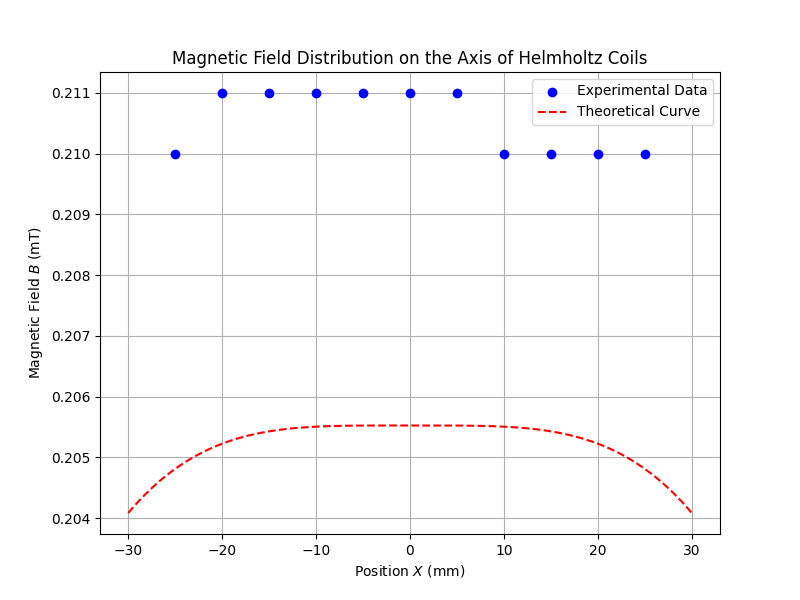
\includegraphics[width=0.8\textwidth]{plot_helmholtz.png}
    \caption{亥姆霍兹线圈轴线上磁感应强度分布}
    \label{fig:helmholtz_dist}
\end{figure}

\textbf{数据分析与误差讨论}：

1. \textbf{磁场均匀性分析}：
根据表 \ref{tab:helmholtz_axial} 及图 \ref{fig:helmholtz_dist} 可知，在亥姆霍兹线圈轴线中心附近区域（$X \in [-10, 10]\,\text{mm}$），磁感应强度 $B$ 的测量值基本保持在 $0.211\,\text{mT}$ 左右，变化极小。这验证了亥姆霍兹线圈在中心附近能产生较大范围均匀磁场的特性，符合实验原理中的描述。

2. \textbf{理论值与测量值的比较}：
根据亥姆霍兹线圈中心磁场公式 \eqref{eq:helmholtz_B_0}，代入参数 $N=400$，$R=0.105\,\text{m}$，$I=60\,\text{mA}=0.060\,\text{A}$，$\mu_0 = 4\pi \times 10^{-7}\,\text{T}\cdot\text{m/A}$，计算理论值为：
\begin{equation}
    B_{\text{理论}} = \left(\frac{4}{5}\right)^{3/2} \frac{\mu_0 N I}{R} \approx 0.7155 \times \frac{4\pi \times 10^{-7} \times 400 \times 0.060}{0.105} \approx 0.2055\,\text{mT}
\end{equation}

取中心附近（$X=0$）的测量值 $B_{\text{实}} = 0.211\,\text{mT}$，则相对误差为：
\begin{equation}
    E = \frac{|B_{\text{实}} - B_{\text{理论}}|}{B_{\text{理论}}} \times 100\% = \frac{|0.211 - 0.2055|}{0.2055} \times 100\% \approx 2.68\%
\end{equation}

3. \textbf{误差来源分析}：
\begin{itemize}
    \item \textbf{线圈几何参数误差}：实际线圈的半径 $R$ 和间距 $a$ 可能与标称值（$105\,\text{mm}$）存在偏差，且两线圈可能不完全平行或共轴，导致磁场分布偏离理论值。
    \item \textbf{电流测量误差}：励磁电流 $I$ 的读数可能存在误差，且电流源的稳定性会影响磁场的稳定性。
    \item \textbf{地磁场影响}：实验测量的磁场较小（约 $0.2\,\text{mT}$），地磁场（约 $0.05\,\text{mT}$）的分量可能会叠加在测量结果中，虽然交流测量模式可以一定程度上消除恒定磁场的影响，但若存在交变干扰磁场仍会产生误差。
    \item \textbf{探测线圈定位误差}：探测线圈可能未完全处于轴线上，或者 $X$ 轴的零点位置存在偏差。
    \item \textbf{频率准确性}：计算公式 $B \propto 1/f$ 依赖于频率 $f$ 的准确性，若实际频率偏离 $120\,\text{Hz}$，会导致计算出的 $B$ 值产生系统误差。
\end{itemize}

\subsection{测量亥姆霍兹线圈径向上磁感应强度的分布}
\begin{table}[htbp]
    \centering
    \caption{亥姆霍兹线圈磁场径向分布测量数据记录 ($f=120\text{Hz}, I=60\text{mA}$)}
    \label{tab:helmholtz_radial}
    \begin{tabular}{cccccccccccc}
        \toprule
        径向距离 $X$ (mm) & -25 & -20 & -15 & -10 & -5 & 0 & 5 & 10 & 15 & 20 & 25 \\
        \midrule
        $U_{max}$ (mV) & 8.62 & 8.63 & 8.64 & 8.64 & 8.64 & 8.64 & 8.64 & 8.62 & 8.62 & 8.61 & 8.61 \\
        测量值 $B$ (mT) & 0.210 & 0.210 & 0.211 & 0.211 & 0.211 & 0.211 & 0.211 & 0.210 & 0.210 & 0.210 & 0.210 \\
        \bottomrule
    \end{tabular}
    
    \vspace{0.5em}
    \footnotesize{注：计算公式为 $B = \frac{2.926}{f} U_{max}$}
\end{table}

\begin{figure}[htbp]
    \centering
    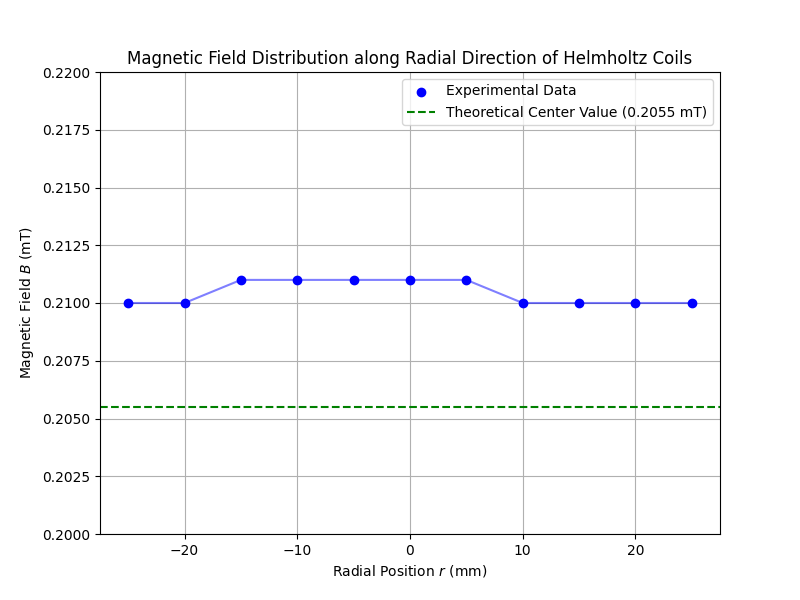
\includegraphics[width=0.8\textwidth]{plot_helmholtz_radial.png}
    \caption{亥姆霍兹线圈磁场径向分布曲线}
    \label{fig:helmholtz_radial}
\end{figure}

\textbf{数据分析与误差讨论}：

1. \textbf{径向均匀性分析}：
根据表 \ref{tab:helmholtz_radial} 及图 \ref{fig:helmholtz_radial} 可知，在亥姆霍兹线圈中心平面的径向方向上，在测量范围 $r \in [-25, 25]\,\text{mm}$ 内，磁感应强度 $B$ 保持高度均匀，数值稳定在 $0.210 \sim 0.211\,\text{mT}$ 之间。这进一步验证了亥姆霍兹线圈在中心区域能够提供高均匀度的磁场环境。

2. \textbf{与理论值的比较}：
径向测量的平均值约为 $0.2105\,\text{mT}$，与轴向测量的中心值 $0.211\,\text{mT}$ 非常接近，且同样略高于理论计算值 $0.2055\,\text{mT}$。相对误差约为：
\begin{equation}
    E = \frac{|0.2105 - 0.2055|}{0.2055} \times 100\% \approx 2.43\%
\end{equation}

3. \textbf{综合误差分析}：
结合轴向和径向的测量结果，实验值普遍略高于理论值（约 $2.5\%$ 的偏差）。除了前述的几何参数误差和地磁场影响外，还可能存在以下系统误差：
\begin{itemize}
    \item \textbf{计算公式系数误差}：实验中使用的计算公式 $B = \frac{2.926}{f} U_{max}$ 中的系数 $2.926$ 是基于特定的线圈参数（如探测线圈的 $NS$ 积）推导而来的。如果探测线圈的实际参数与标称值有出入，将直接导致计算结果的系统性偏差。
    \item \textbf{频率 $f$ 的波动}：实验中假设频率恒定为 $120\,\text{Hz}$，若实际驱动信号频率略低于该值，会导致计算出的 $B$ 值偏大。
    \item \textbf{仪器定标误差}：数字毫伏表或磁感应强度测量仪的内部定标可能存在微小偏差。
\end{itemize}

\subsubsection{探测线圈转角与感应电压}
\begin{table}[htbp]
    \centering
    \caption{探测线圈转角与感应电压数据记录 ($f=120\text{Hz}, I=60\text{mA}$)}
    \label{tab:coil_rotation}
    \setlength{\tabcolsep}{4pt} % 减小列间距
    
    % 第一部分 0-90度
    \begin{tabular}{ccccccccccc}
        \toprule
        探测线圈转角 $\theta (^\circ)$ & 0 & 10 & 20 & 30 & 40 & 50 & 60 & 70 & 80 & 90 \\
        \midrule
        $U (\text{mV})$ & 8.64 & 8.52 & 8.09 & 7.48 & 6.67 & 5.50 & 4.28 & 2.81 & 1.38 & 0.00 \\
        计算值: $U_{max}\cos\theta$ & 8.64 & 8.51 & 8.12 & 7.48 & 6.62 & 5.55 & 4.32 & 2.96 & 1.50 & 0.00 \\
        \bottomrule
    \end{tabular}

    \vspace{1em}

    % 第二部分 100-190度
    \begin{tabular}{ccccccccccc}
        \toprule
        探测线圈转角 $\theta (^\circ)$ & 100 & 110 & 120 & 130 & 140 & 150 & 160 & 170 & 180 & 190 \\
        \midrule
        $U (\text{mV})$ & 1.57 & 3.05 & 4.38 & 5.56 & 6.67 & 7.55 & 8.12 & 8.52 & 8.67 & 8.48 \\
        计算值: $|U_{max}\cos\theta|$ & 1.50 & 2.96 & 4.32 & 5.55 & 6.62 & 7.48 & 8.12 & 8.51 & 8.64 & 8.51 \\
        \bottomrule
    \end{tabular}

    \vspace{1em}

    % 第三部分 200-290度
    \begin{tabular}{ccccccccccc}
        \toprule
        探测线圈转角 $\theta (^\circ)$ & 200 & 210 & 220 & 230 & 240 & 250 & 260 & 270 & 280 & 290 \\
        \midrule
        $U (\text{mV})$ & 8.19 & 7.62 & 6.73 & 5.61 & 4.27 & 2.98 & 1.60 & 0.10 & 1.35 & 2.91 \\
        计算值: $|U_{max}\cos\theta|$ & 8.12 & 7.48 & 6.62 & 5.55 & 4.32 & 2.96 & 1.50 & 0.00 & 1.50 & 2.96 \\
        \bottomrule
    \end{tabular}

    \vspace{1em}

    % 第四部分 300-360度
    \begin{tabular}{ccccccccc}
        \toprule
        探测线圈转角 $\theta (^\circ)$ & 300 & 310 & 320 & 330 & 340 & 350 & 360 & \\
        \midrule
        $U (\text{mV})$ & 4.24 & 5.47 & 6.47 & 7.41 & 8.07 & 8.49 & 8.64 & \\
        计算值: $|U_{max}\cos\theta|$ & 4.32 & 5.55 & 6.62 & 7.48 & 8.12 & 8.51 & 8.64 & \\
        \bottomrule
    \end{tabular}
    
    \vspace{0.5em}
    \footnotesize{注：计算中使用 $U_{max} = U(0^\circ) = 8.64 \text{mV}$。由于测量值为电压幅值，计算公式取绝对值。}
\end{table}

\begin{figure}[htbp]
    \centering
    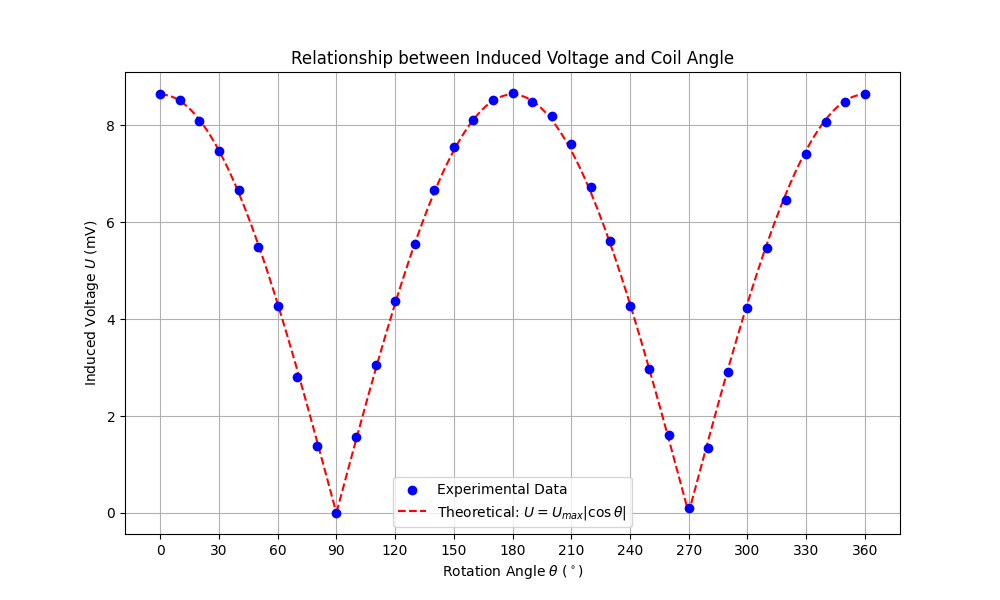
\includegraphics[width=0.8\textwidth]{plot_coil_rotation.png}
    \caption{探测线圈感应电压随转角变化曲线}
    \label{fig:coil_rotation}
\end{figure}

\textbf{数据分析与误差讨论}：

1. \textbf{验证余弦关系}：
根据电磁感应原理，感应电动势的幅值 $\varepsilon_m \propto \cos\theta$。由于实验测量的是电压有效值（或幅值），且不区分正负（交流电压表读数为正值），理论上应满足 $U = U_{max} |\cos\theta|$。
从图 \ref{fig:coil_rotation} 可以看出，实验测量点（蓝色散点）与理论余弦曲线（红色虚线）吻合度极高。

2. \textbf{误差分析}：
计算实验值与理论值的平均绝对误差（MAE）约为 $0.0587\,\text{mV}$，相对于最大电压 $8.64\,\text{mV}$，平均相对误差仅为 $0.68\%$。这表明实验结果非常好地验证了 $\varepsilon_m(\theta) = N S B_m \omega \cos\theta$ 这一关系式。
微小的误差可能来源于：
\begin{itemize}
    \item \textbf{角度读取误差}：转动装置的角度刻度可能存在读数视差或机械回差。
    \item \textbf{初始位置偏差}：$0^\circ$ 的初始位置可能未完全对准磁场方向（即线圈法线与磁场方向未完全重合）。
    \item \textbf{背景噪声}：在电压较小（如 $90^\circ$ 和 $270^\circ$ 附近）时，环境电磁干扰或仪器底噪可能对测量结果产生较大影响（例如 $270^\circ$ 时测量值为 $0.10\,\text{mV}$ 而非 $0$）。
\end{itemize}

\subsubsection{励磁电流频率大小对磁感应强度的影响}
\begin{table}[htbp]
    \centering
    \setlength{\tabcolsep}{3.5pt} % 调整列间距
    \caption{励磁电流频率对磁场强度的影响 ($I=60\text{mA}$)}
    \label{tab:frequency_effect}
    \begin{tabular}{lccccccccccc}
        \toprule
        励磁电流频率 $f$ (Hz) & 20 & 30 & 40 & 50 & 60 & 70 & 80 & 90 & 100 & 110 & 120 \\
        \midrule
        $U_{max}$ (mV) & 1.44 & 2.13 & 2.87 & 3.63 & 4.29 & 4.98 & 5.71 & 6.43 & 7.13 & 7.84 & 8.63 \\
        测量值 $B$ (mT) & 0.211 & 0.208 & 0.210 & 0.212 & 0.209 & 0.208 & 0.209 & 0.209 & 0.209 & 0.209 & 0.210 \\
        \bottomrule
    \end{tabular}
    
    \vspace{0.5em}
    \footnotesize{注：计算公式为 $B = \frac{2.926}{f} U_{max}$，实验中始终保持励磁电流 $I=60\text{mA}$。}
\end{table}

\begin{figure}[htbp]
    \centering
    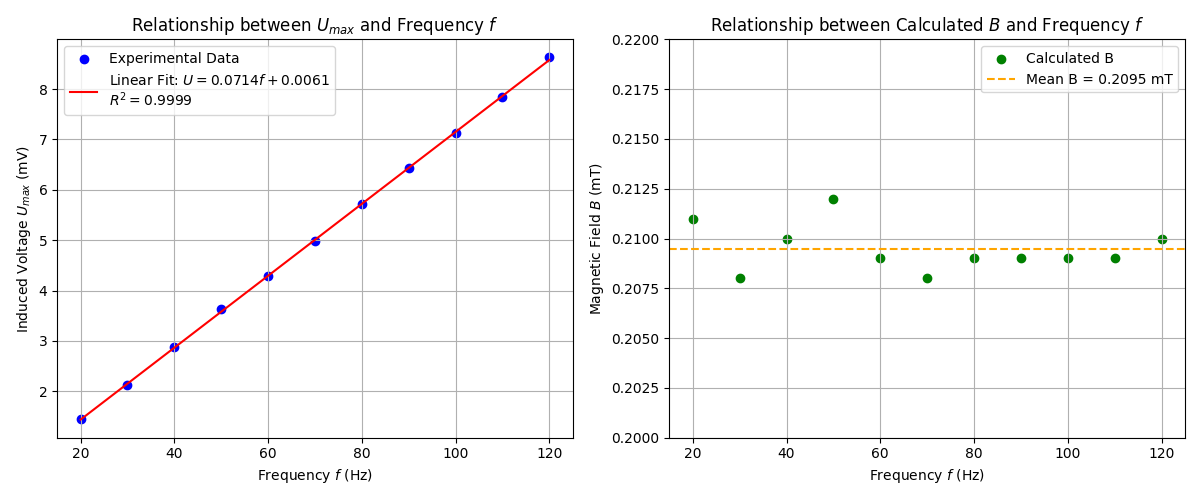
\includegraphics[width=\textwidth]{plot_frequency_effect.png}
    \caption{感应电压 $U_{max}$ 及磁感应强度 $B$ 随频率 $f$ 的变化关系}
    \label{fig:frequency_effect}
\end{figure}

\textbf{数据分析与误差讨论}：

1. \textbf{感应电压与频率的关系}：
由图 \ref{fig:frequency_effect} 左图可知，在励磁电流恒定 ($I=60\,\text{mA}$) 的情况下，探测线圈的感应电压 $U_{max}$ 与频率 $f$ 呈现极好的线性关系。线性拟合结果显示 $R^2 \approx 0.9999$，且截距几乎为零。这完美验证了法拉第电磁感应定律：感应电动势 $\varepsilon \propto \frac{d\Phi}{dt} \propto \omega B \propto f$。

2. \textbf{磁感应强度与频率的关系}：
由图 \ref{fig:frequency_effect} 右图可知，根据公式 $B = \frac{C}{f} U_{max}$ 计算得到的磁感应强度 $B$ 在 $20 \sim 120\,\text{Hz}$ 的频率范围内基本保持恒定，平均值为 $0.2095\,\text{mT}$，标准差仅为 $0.0012\,\text{mT}$。这说明亥姆霍兹线圈产生的磁场大小主要取决于励磁电流的大小，而在低频范围内与频率无关。

3. \textbf{综合结论}：
实验结果表明，利用电磁感应法测量交变磁场时，必须准确知道信号的频率，或者使用具有频率补偿功能的测量仪器。同时，实验测得的 $B$ 值 ($0.2095\,\text{mT}$) 与前述轴向分布测量中的中心值 ($0.211\,\text{mT}$) 高度一致，进一步验证了实验数据的可靠性。

\section{思考题回答}

\subsection{手机能不能改变地球磁场？怎么改变的？}

严格来说，手机\textbf{不能改变地球本身的内源磁场}，但\textbf{可以改变手机周围局部的磁场分布}。

首先，我们需要区分“地球磁场”这一概念的宏观与微观定义。地球磁场（Geomagnetic field）主要源于地球内部液态外核的“发电机效应”，这是一个全球性的、巨大的磁场，其强度在地表约为 $25 \sim 65\, \mu\text{T}$（即 $2.5 \times 10^{-5} \sim 6.5 \times 10^{-5}\,\text{T}$）。手机作为一个微小的电子设备，其能量完全不足以影响地球内部的物理过程，因此不可能从根本上改变地球磁场的产生机制或整体形态。

然而，在微观和局部范围内，手机确实会通过\textbf{磁场叠加原理}改变其周围空间的磁感应强度矢量。这主要通过以下两种方式实现：

\begin{enumerate}
    \item \textbf{硬磁性材料的干扰}：手机内部含有多种永久磁铁部件，例如扬声器、听筒、振动马达以及摄像头的对焦模组，甚至部分手机背面用于无线充电定位的磁环（如 MagSafe）。这些部件具有恒定的磁矩，会在其周围产生静磁场。当这个磁场与地磁场共存时，根据矢量叠加原理，空间中某点的总磁场 $\vec{B}_{\text{total}} = \vec{B}_{\text{earth}} + \vec{B}_{\text{phone}}$。在手机紧邻的区域，$\vec{B}_{\text{phone}}$ 的强度甚至可能远超地磁场，导致该处的磁力线发生扭曲。
    \item \textbf{电流产生的电磁场}：手机在工作时，内部的印刷电路板（PCB）、天线和处理器中有电流通过。根据安培定律和毕奥-萨伐尔定律，变化的电流会在周围激发变化的电磁场。虽然这种场通常较弱且随距离衰减极快，但它依然是对局部电磁环境的一种改变。
\end{enumerate}

综上所述，手机虽然无法撼动地球磁场的根本，但它就像河流中的一块石头，会改变经过它周围的“水流”（磁力线）的走向。这也正是为什么我们在使用手机指南针时，往往需要进行“8字形”校准，其目的就是为了让传感器计算并扣除手机自身软硬磁性材料产生的“局部磁场偏差”，从而还原出真实的地球北极方向。

\subsection{地球磁鞘有什么用？没有会发生什么？}

\textbf{地球磁鞘（Magnetosheath）的作用：}
地球磁鞘是位于地球弓形激波（Bow Shock）和磁层顶（Magnetopause）之间的湍流等离子体区域。它的主要作用是作为一个\textbf{缓冲区}或\textbf{减速带}。当超声速的太阳风粒子流撞击地球磁层时，首先在弓形激波处急剧减速、压缩并加热，从超声速变为亚声速，然后进入磁鞘区域，最後由磁鞘引导这些粒子流绕过地球磁层流向后方。

\textbf{如果没有地球磁鞘（即没有磁层的保护）会发生什么：}
如果不存在这种保护机制（类似于火星的情况），后果将是灾难性的：
\begin{itemize}
    \item \textbf{大气层剥离}：高能太阳风将直接轰击地球大气层，像剥洋葱一样将大气分子电离并吹向太空，导致地球大气层逐渐变薄甚至消失，液态水也将无法存在。
    \item \textbf{致命辐射}：地表将直接暴露在强烈的宇宙射线和太阳高能粒子流之下，这将摧毁生物的 DNA，导致地球表面不再适合生命生存。
    \item \textbf{电磁设施瘫痪}：对于现代人类社会，没有磁层和磁鞘的缓冲，所有的卫星、电网和通信系统都将在太阳风暴面前不堪一击，瞬间瘫痪。
\end{itemize}

\subsection{从人类大脑到电磁铁 $10^{-5} \rightarrow 10^1\,\text{T}$ 对人类有什么影响}

这个问题涉及磁场强度跨越多个数量级时对人体产生的不同生物物理效应。

\begin{enumerate}
    \item \textbf{低场强区间 ($10^{-5}\,\text{T}$ 量级) - 地磁场水平}：\\
    地球表面的背景磁场约为 $50\,\mu\text{T}$ ($5 \times 10^{-5}\,\text{T}$)。人类大脑自身的神经活动也会产生极微弱的磁场（飞特斯拉 $10^{-15}\,\text{T}$ 级别，需用 SQUID 探测）。
    \begin{itemize}
        \item \textbf{影响}：在这个量级下，对人体\textbf{无明显影响}。人类是在地磁场环境中进化的，对此完全适应。
    \end{itemize}

    \item \textbf{中场强区间 ($10^{-3} \sim 10^{-1}\,\text{T}$) - 普通磁铁}：\\
    生活中常见的强力磁铁或工业环境。
    \begin{itemize}
        \item \textbf{影响}：通常认为是安全的。但对于植入心脏起搏器或体内有铁磁性植入物的人群，可能会造成设备故障或植入物移位。
    \end{itemize}

    \item \textbf{高场强区间 ($10^0 \sim 10^1\,\text{T}$) - 强电磁铁/MRI}：\\
    医用核磁共振（MRI）通常为 $1.5\,\text{T}$ 或 $3.0\,\text{T}$，科研用强磁场可达 $10\,\text{T}$ 以上。
    \begin{itemize}
        \item \textbf{磁光幻视 (Phosphenes)}：当头部在强磁场中快速移动时，视网膜受到磁场感应电流的刺激，人会看到闪光。
        \item \textbf{眩晕与恶心}：强磁场作用于内耳半规管中的淋巴液（含有带电离子），产生的洛伦兹力会导致“磁性眩晕感”和平衡失调。
        \item \textbf{心血管效应}：在 $10\,\text{T}$ 这种极端磁场下，血液流动（导电液体在磁场中运动）可能会产生显著的霍尔电压，理论上可能轻微影响心电图信号，但短期暴露通常无永久性损伤。
    \end{itemize}
\end{enumerate}

\textbf{总结}：从 $10^{-5}\,\text{T}$ 到 $10^1\,\text{T}$，磁场对人的影响从“完全无感”逐渐变为“产生感应电流导致的神经刺激（眩晕、闪光）”，只要没有金属植入物，静磁场本身在 $10^1\,\text{T}$ 以下通常不会造成永久性的生物组织损伤。

\section{实验讨论}

在本次实验中，我们通过多种方法测量了磁场的分布和强度，并验证了理论模型的正确性。然而，在实验过程中仍然存在一些问题和改进空间：

\subsection{实验中存在的问题}
\begin{enumerate}
    \item \textbf{测量误差}：由于仪器的分辨率有限以及环境磁场的干扰，测量数据中存在一定的随机误差和系统误差。例如，在测量霍尔电压时，可能受到温度变化的影响。
    \item \textbf{数据拟合偏差}：在某些实验中，数据点的分布未完全符合理论曲线，可能是由于实验操作中的不确定性或模型假设的简化。
    \item \textbf{重复性问题}：部分实验的重复性较差，可能与实验条件的控制不够严格有关，例如线圈电流的稳定性和传感器的校准。
\end{enumerate}

\subsection{进一步的想法}
\begin{enumerate}
    \item \textbf{提高仪器精度}：使用更高精度的电流源和电压表，减少测量误差的来源。同时，增加屏蔽措施以降低环境磁场的干扰。
    \item \textbf{改进实验方法}：在数据采集过程中，采用多次测量取平均值的方法，以提高数据的可靠性。此外，可以尝试使用更先进的传感器，例如基于光学原理的磁场测量设备。
    \item \textbf{扩展实验内容}：进一步研究不同频率的交变磁场对霍尔效应的影响，或者探索更高强度磁场下的物理现象，例如磁饱和效应。
    \item \textbf{理论模型优化}：结合实验数据，优化理论模型的参数，或者引入更复杂的数学模型以解释实验中的偏差。
\end{enumerate}

通过以上改进和扩展，可以进一步提高实验的精度和科学价值，为后续研究提供更可靠的数据支持。

\section{原始实验数据记录表格}
\begin{figure}
    \centering
    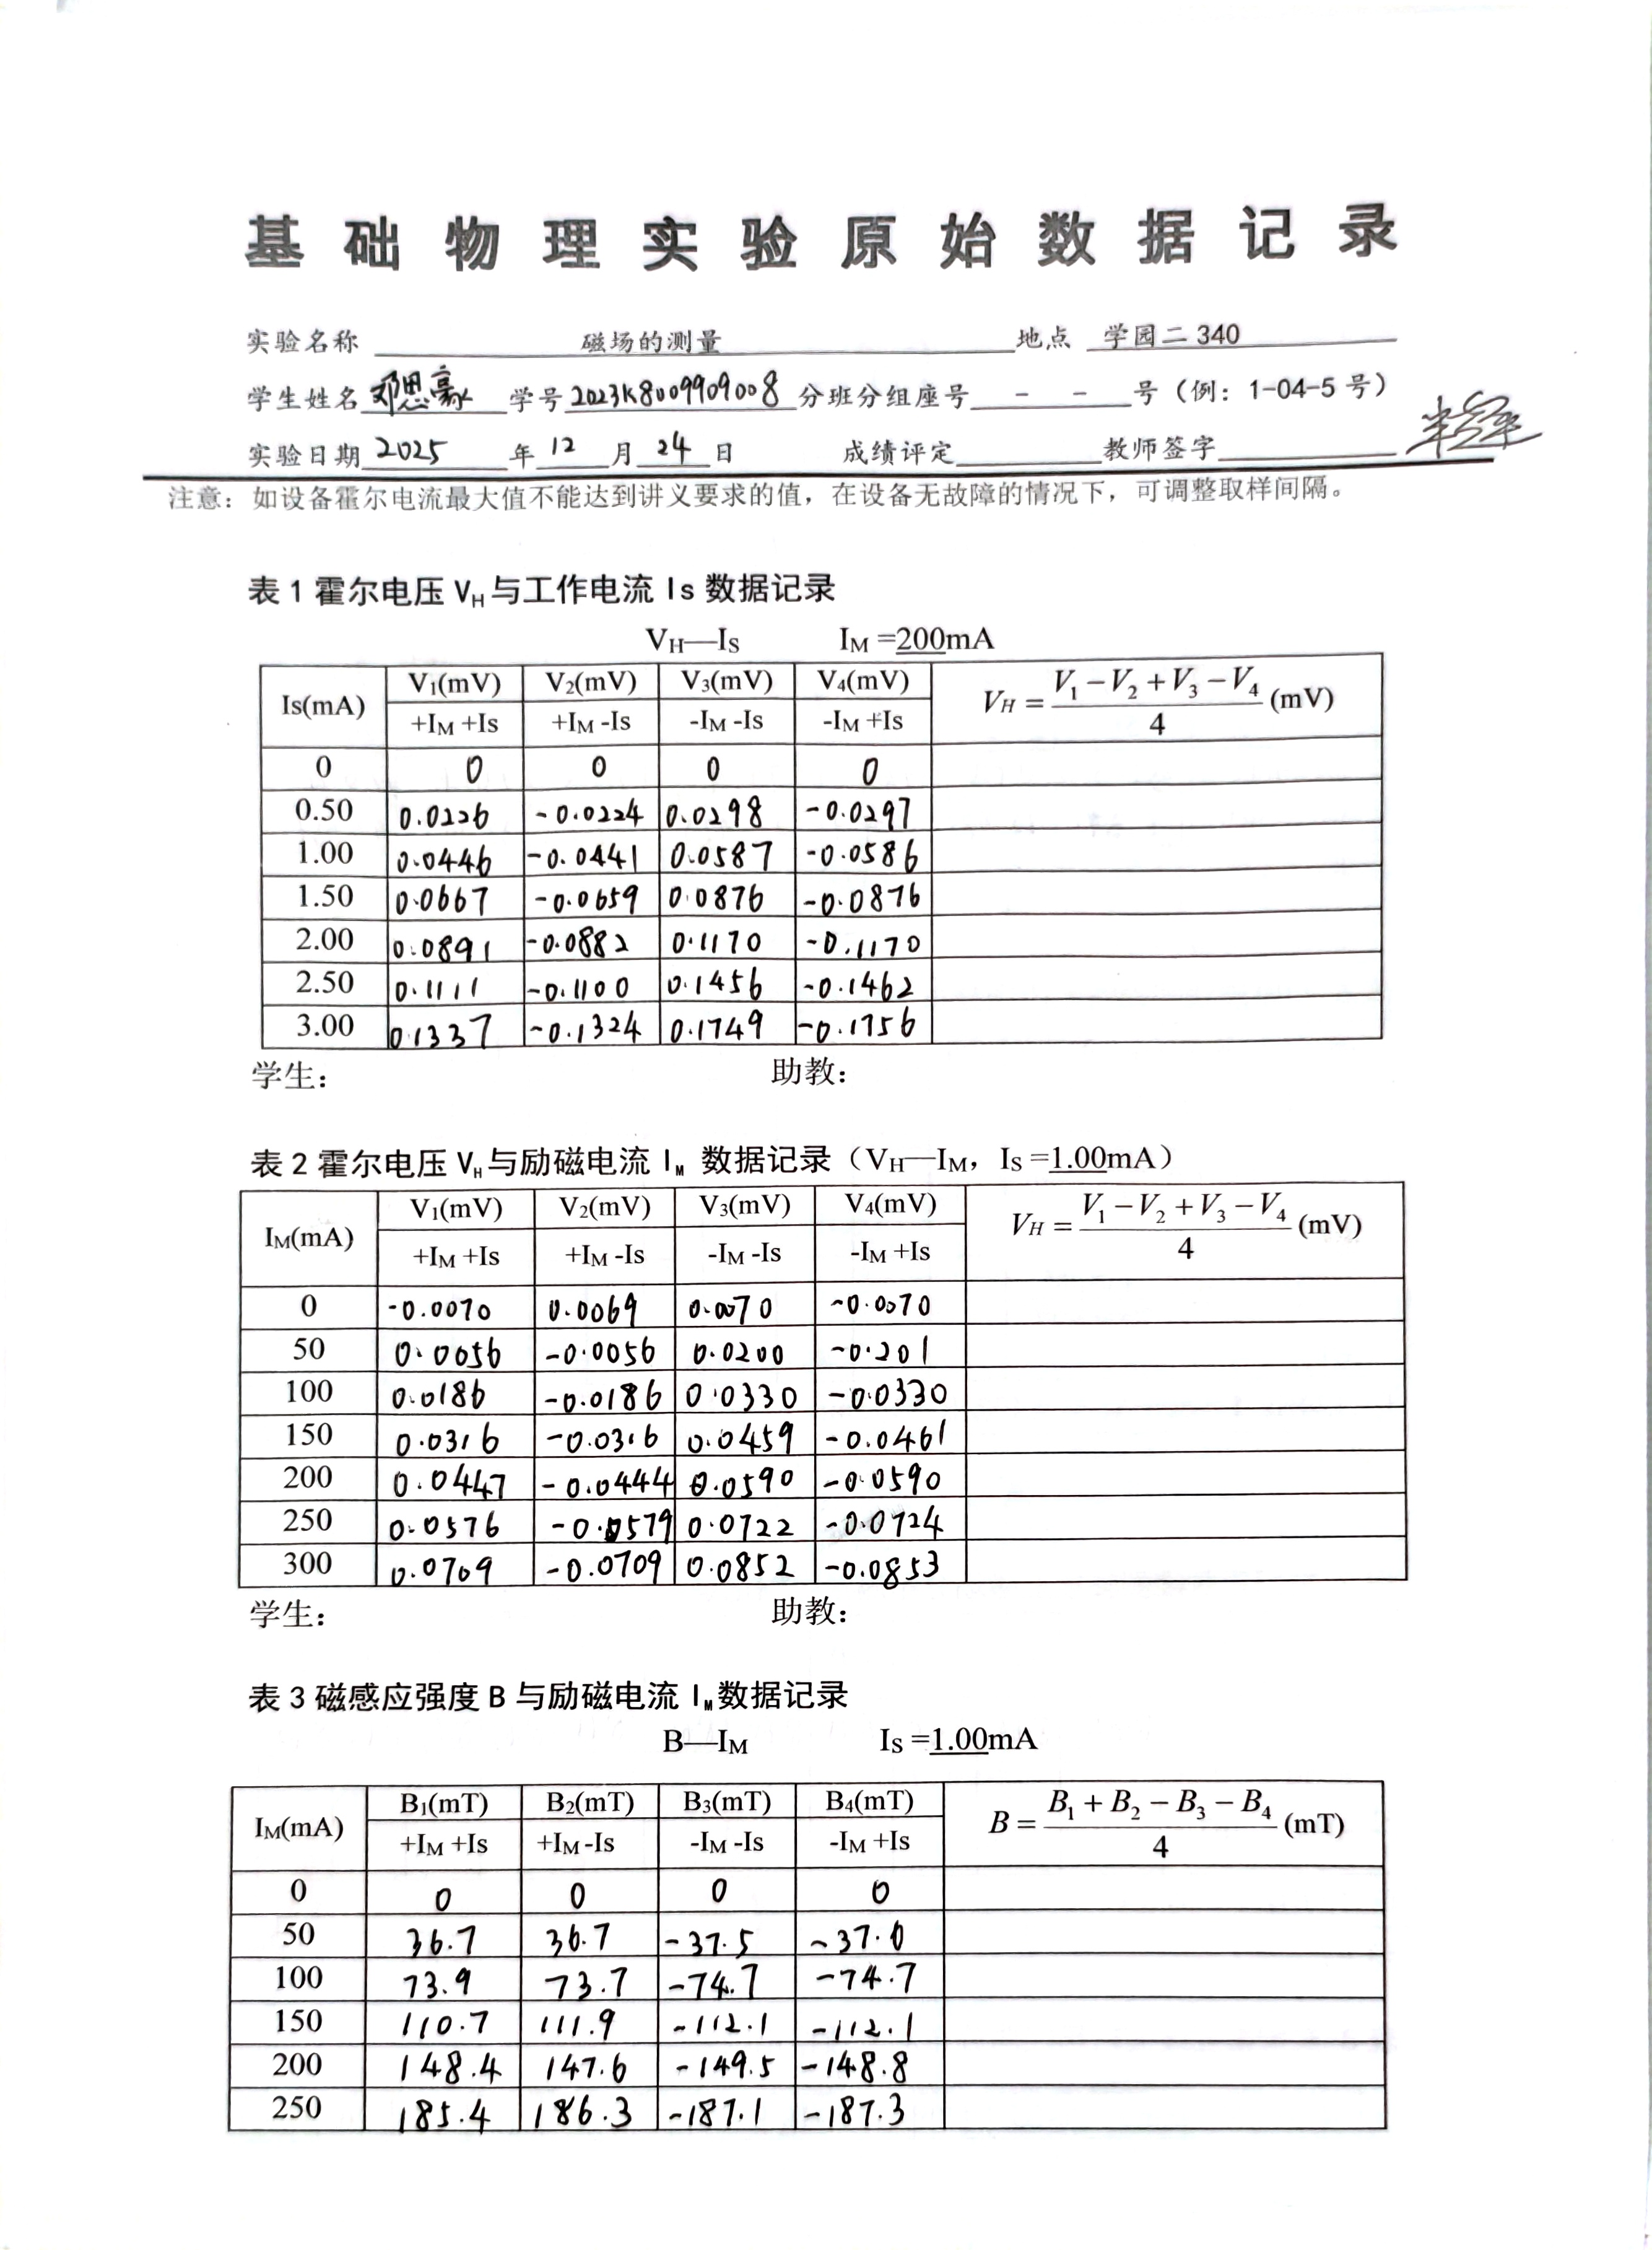
\includegraphics[width=\textwidth]{raw_data_1.jpg}
    \caption{实验数据记录表格1}
    \label{fig:raw_data_1}
\end{figure}
\begin{figure}
    \centering
    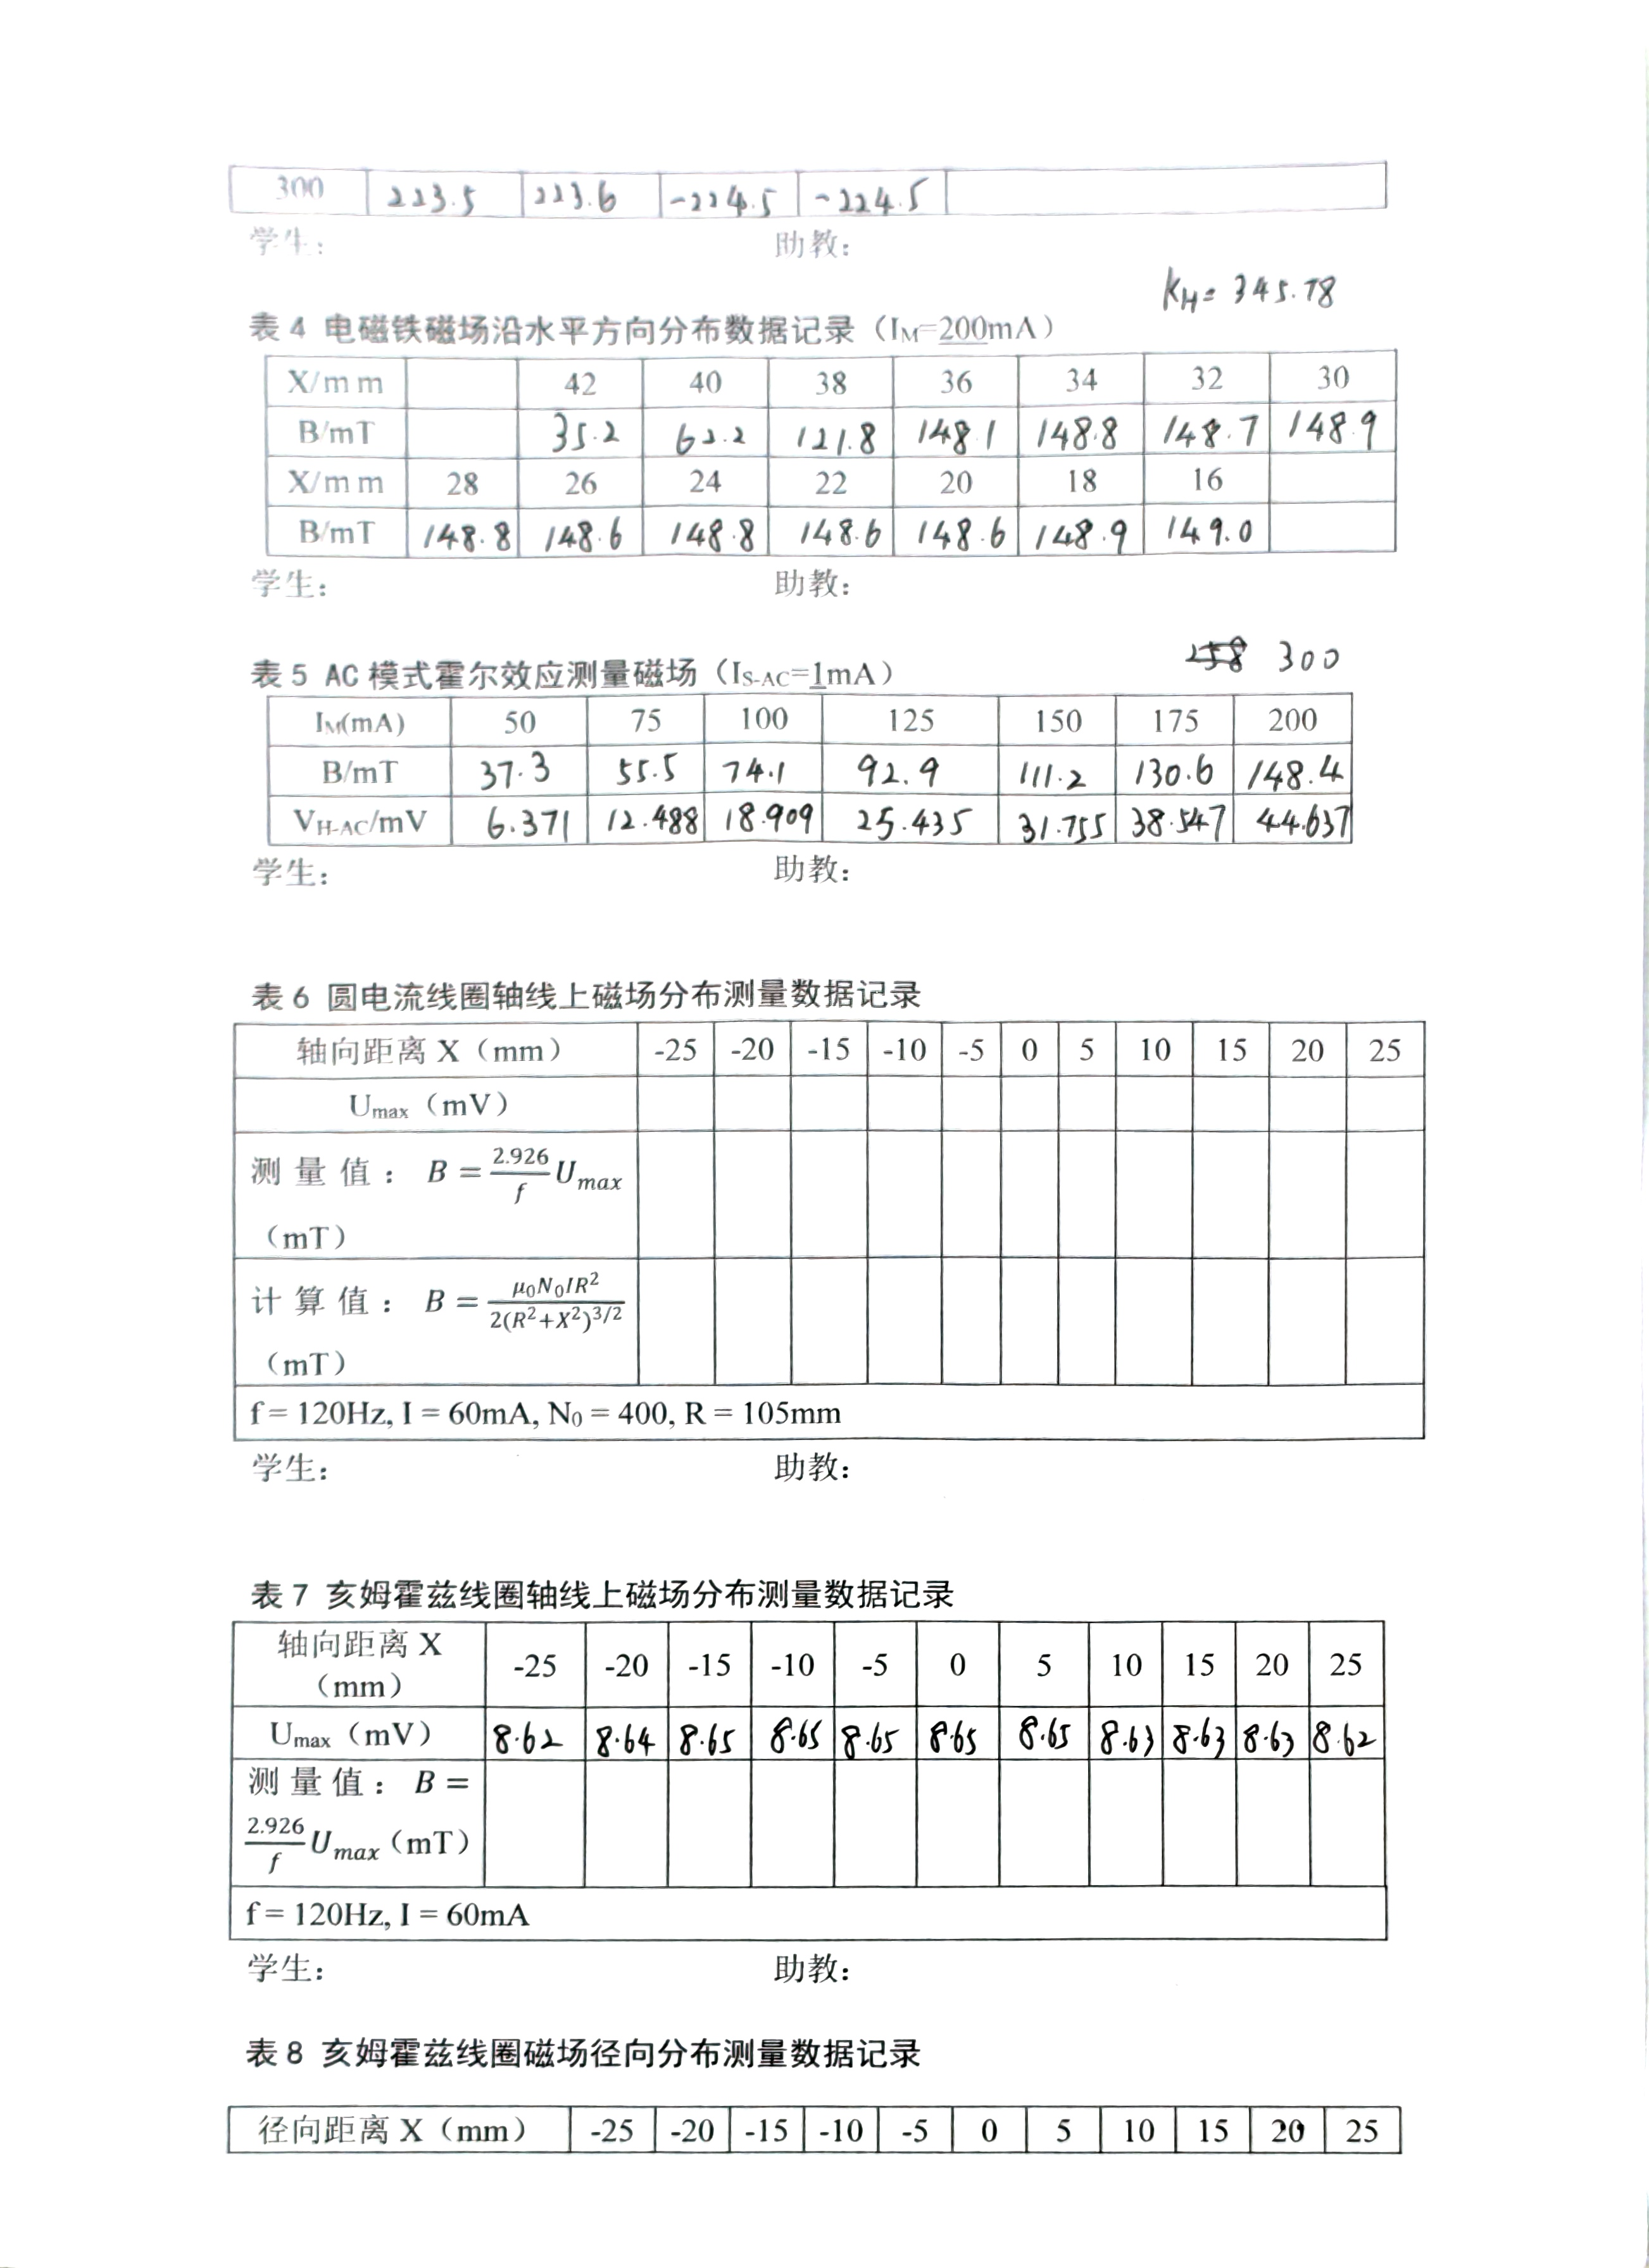
\includegraphics[width=\textwidth]{raw_data_2.jpg}
    \caption{实验数据记录表格2}
    \label{fig:raw_data_2}
\end{figure}
\begin{figure}
    \centering
    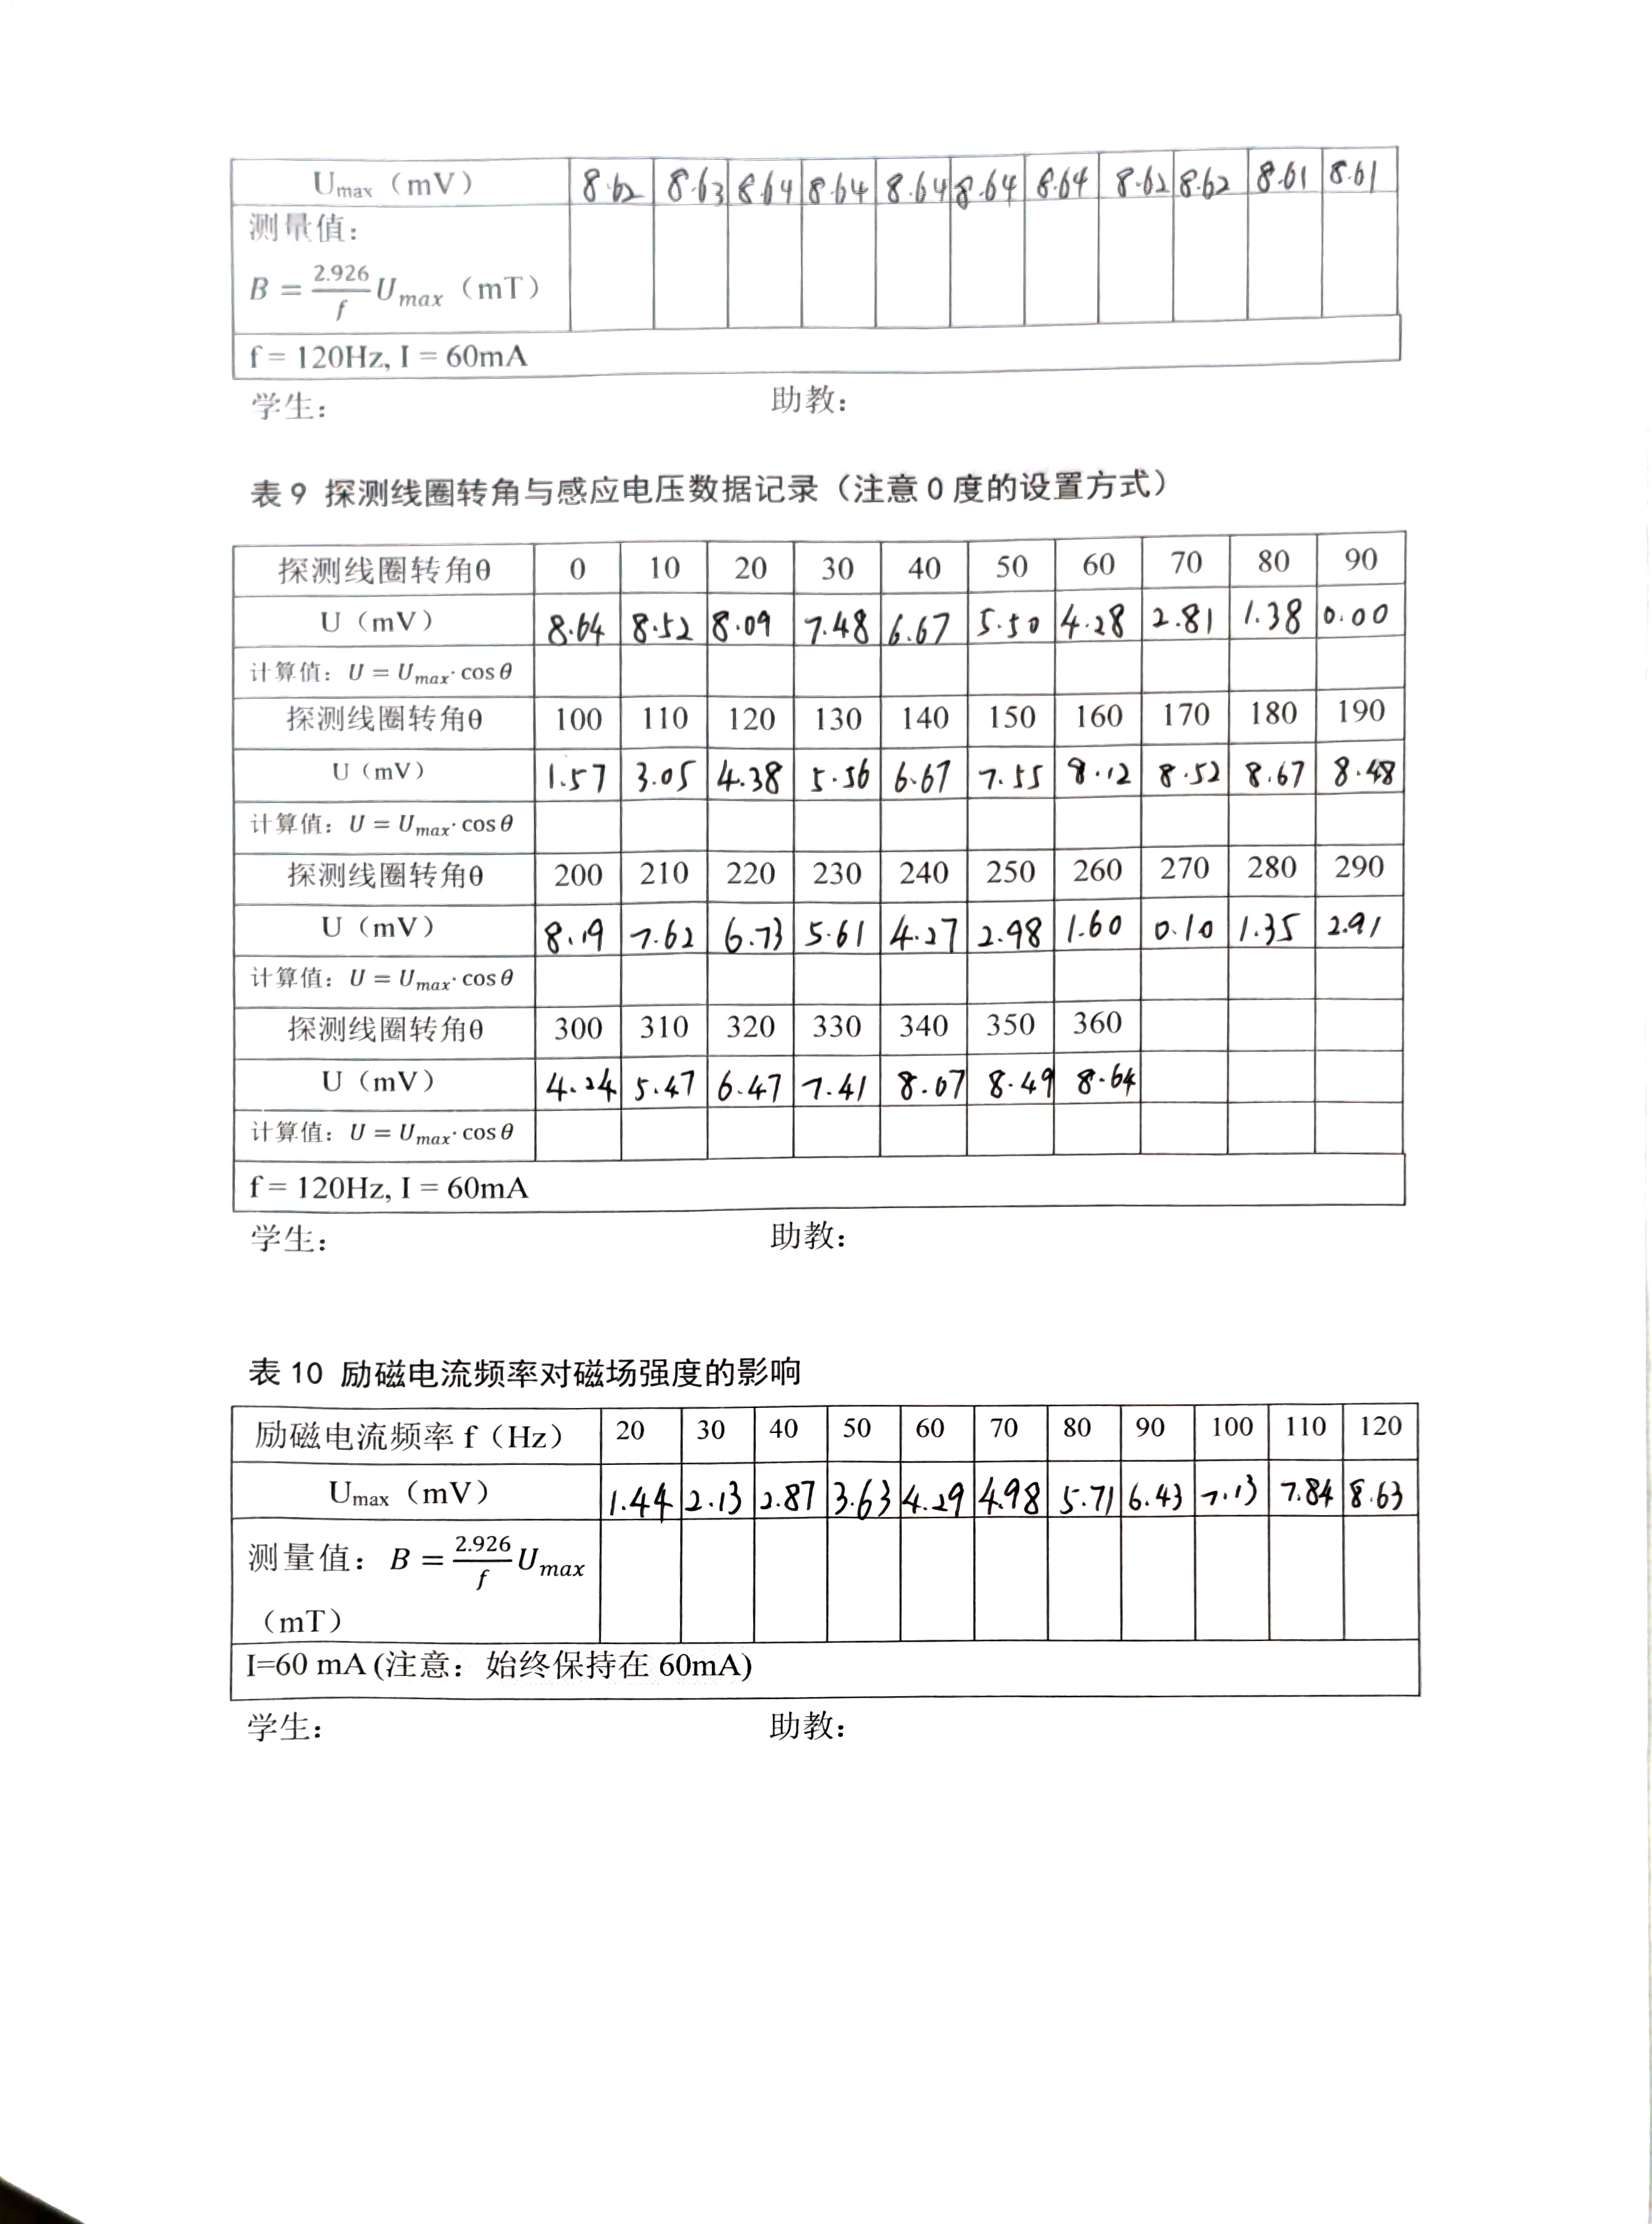
\includegraphics[width=\textwidth]{raw_data_3.jpg}
    \caption{实验数据记录表格3}
    \label{fig:raw_data_3}
\end{figure}
\end{document}